%%%%%%%%%%%%%%%%%%%%%%%%%%%%%%%%%%%%%%%%%%%%%%%%%%%%%%%%%%%%
%2345678901234567890123456789012345678901234567890123456789012345678901234567890
%        1         2         3         4         5         6         7         8

\documentclass[letterpaper, 10 pt, conference]{ieeeconf}  % Comment this line out
                                                          % if you need a4paper
%\documentclass[a4paper, 10pt, conference]{ieeeconf}      % Use this line for a4
                                                          % paper

\IEEEoverridecommandlockouts                              % This command is only
                                                          % needed if you want to
                                                          % use the \thanks command
\overrideIEEEmargins
% See the \addtolength command later in the file to balance the column lengths
% on the last page of the document



% The following packages can be found on http:\\www.ctan.org
%\usepackage{graphics} % for pdf, bitmapped graphics files
%\usepackage{epsfig} % for postscript graphics files
%\usepackage{mathptmx} % assumes new font selection scheme installed
%\usepackage{times} % assumes new font selection scheme installed
%\usepackage{amsmath} % assumes amsmath package installed
%\usepackage{amssymb}  % assumes amsmath package installed
\usepackage{graphicx}
\usepackage{verbatim}
\usepackage{multirow}
\usepackage{rotating}
\usepackage{moreverb}                    % for boxedboxedverbatim
\usepackage{array}
\usepackage{fancyvrb}
\usepackage{multicol}
\usepackage{mdwlist}
\usepackage{enumerate}
%\usepackage{tikz-er2}


\newtheorem{defn}{Definition}

\newcommand{\class}[1] {\textit{#1}}
\newcommand{\const}[1] {$\mathit{#1}$}
\newcommand{\objvar}[1] {$\mathsf{#1}$}
\newcommand{\stvar}[1] {\textsf{#1}}
\newcommand{\op}[1] {\textsl{#1}}
\newcommand{\nil} {\textit{nil}\ }

\newcommand\T{\rule{0pt}{2.6ex}}
\newcommand\B{\rule[-1.2ex]{0pt}{0pt}}

%\definecolor{violetred}{cmyk}{0,0.85,0.31,0.18}
%\definecolor{darkblue}{cmyk}{1,1,0,0.45}
%\definecolor{lavenderblush4}{cmyk}{0,0.06,0.04,0.45}
%\definecolor{packergreen}{cmyk}{0.46,0,0.21,0.76}
%\definecolor{fuschia}{cmyk}{0,100,0,0}
%\definecolor{graycmyk}{cmyk}{0,0,0,0.74}
%
%\usetikzlibrary{calc,trees,positioning,arrows,chains,shapes.geometric,%
%    decorations.pathreplacing,decorations.pathmorphing,shapes,%
%    matrix,shapes.symbols,positioning,shadows}
%
%% styles for flowcharts
%
%\tikzstyle{every entity} = [top color=white, bottom color=blue!30,
%                            draw=blue!50!black!100, drop shadow]
%\tikzstyle{empty} = [top color=white, bottom color=white,
%                            draw=white]
%
%\tikzstyle{every weak entity} = [drop shadow={shadow xshift=.7ex,
%                                 shadow yshift=-.7ex}]
%\tikzstyle{every attribute} = [top color=white, bottom color=green!20,
%                               draw=green, node distance=1cm, drop shadow]
%\tikzstyle{ELLIPSE} = [draw, ellipse, top color=white, bottom color=green!20, draw=green, drop shadow]
%\tikzstyle{MainAttribute} = [draw, rectangle,top color=white, bottom color=red!20,
%                               draw=red, node distance=1cm, drop shadow]
%\tikzstyle{DATABASE} = [draw, rectangle, rounded corners,top color=white, bottom color=graycmyk!50, draw=graycmyk, inner sep=10pt, drop shadow={shadow xshift=.7ex, shadow yshift=-.7ex}]
%
%
%\tikzstyle{myarrow}=[->, >=stealth', thick, shorten <=2pt,shorten >=2pt]
%
%
%
%\tikzstyle{output} = [draw, rectangle, rounded corners,top color=white, bottom color=red!30, draw=red, inner sep=10pt, drop shadow={shadow xshift=.7ex, shadow yshift=-.7ex}]
%
%\tikzstyle{abstract}=[rectangle, draw=black, rounded corners, fill=blue!40, drop shadow,
%        text centered, anchor=north, text=white, text width=3cm]
%
%
%\newbox{\LegendOutput}
%\savebox{\LegendOutput}{
%    (\begin{tikzpicture}[]
%    \node[output] (2) {\hspace{5 mm}};
%    \end{tikzpicture}
%    )}


\newenvironment{mylisting}
{\begin{list}{}{\setlength{\leftmargin}{1em}}\item\small}
{\end{list}}

\newenvironment{mytinylisting}
{\begin{list}{}{\setlength{\leftmargin}{1em}}\item\tiny\bfseries}
{\end{list}}


\title{\LARGE \bf
Metrics and Test Methods for Industrial Kit Building
}

%\author{ \parbox{3 in}{\centering Stephen Balakirsky\\
%         Intelligent Systems Division\\
%         National Institute of Standards and Technology\\
%        Gaithersburg, MD 20899, USA\\
%         {\tt\small stephen.balakirsky@nist.gov}}
%         \hspace*{ 0.5 in}
%         \parbox{3 in}{ \centering Zeid Kootbally\\
%          Department of Mechanical Engineering \\
%         University of Maryland\\
%         College Park, MD 20742, USA\\
%         {\tt\small zeid.kootbally@nist.gov}}\\ \\
%	\parbox{2.25 in}{\centering Craig Schlonoff\\
%         Intelligent Systems Division\\
%         National Institute of Standards and Technology\\
%        Gaithersburg, MD 20899, USA\\
%         {\tt\small craig.schlenoff@nist.gov}}
%        \hspace*{0.05in}
%         \parbox{2.25 in}{ \centering Thomas Kramer\\
%          Department of Mechanical Engineering \\
%         Catholic University of America\\
%         Washington, DC 20064, USA\\
%         {\tt\small thomas.kramer@nist.gov}}
%        \hspace*{0.05in}
%         \parbox{2.25 in}{ \centering Satyandra K. Gupta\\
%          Maryland Robotics Center\\
%         University of Maryland\\
%         College Park, MD 20742, USA\\
%         {\tt\small skgupta@umd.edu}}\\
%}

\author{Stephen Balakirsky, Thomas Kramer, and Zeid Kootbally% <-this % stops a space
\thanks{S. Balakirsky is with the Intelligent Systems Division, National Institute of Standards and Technology, Gaithersburg, MD, USA (e-mail:stephen.balakirsky@nist.gov)}% <-this % stops a space
\thanks{Z. Kootbally is with the Department of Mechanical Engineering, University of Maryland, College Park, MD, USA (email: zeid.kootbally@nist.gov)}%
\thanks{T. Kramer is with the Department of Mechanical Engineering, Catholic University of America, Washington, DC, USA (email: thomas.kramer@nist.gov)}%
} 


\begin{document}
%\begin {center}
{\huge{Outline}}
\end {center}

\begin{enumerate}
\item SB - Description of kitting
\item Test methods
	\begin{enumerate}
	\item TK -  Inputt format (xml, owl)
	\item TK - Output format (Robot canonical command language)
	\item SB - method itself (build kits) with varying part mix and configuration, missing parts, ...
	\end{enumerate}
\item metrics
	\begin{enumerate}
	\item TK -  Plan
		\begin{enumerate}
		\item number of steps
		\item goal achievement
		\item optimality
		\item maintain constraints
		\item number of errors
		\end {enumerate}
	\item ZK -  Execution
	\end {enumerate}
\item assumptions
	\begin {enumerate}
	\item Work volume totally reachable
	\end {enumerate}
\end{enumerate}


\maketitle
\thispagestyle{empty}
\pagestyle{plain}
\pagenumbering{arabic}

%%%%%%%%%%%%%%%%%%%%%%%%%%%%%%%%%%%%%%%%%%%%%%%%%%%%%%%%%%%%
\begin{abstract}

The IEEE RAS Ontologies for Robotics and Automation Working Group is dedicated to
developing a methodology for knowledge representation and reasoning in robotics
and automation. As part of this working group, the Industrial Robots sub-group is
tasked with studying industrial applications of the knowledge representation. One of the first
areas of interest for this subgroup is the area of kit building or kitting.
It is anticipated that utilization of the knowledge representation will allow for the development
of higher performing kitting systems. However, the definition of ``higher performing''
has yet to be defined. This paper addresses this issue by providing the basis
for performance methods and metrics that are designed to
determine the performance of a kitting system.
\end{abstract}


%%%%%%%%%%%%%%%%%%%%%%%%%%%%%%%%%%%%%%%%%%%%%%%%%%%%%%%%%%%%
\section{INTRODUCTION}
Material feeding systems are an integral part of today's assembly line operations.
These systems assure that parts are available where and when
they are needed during the assembly operations by providing either a continuous
supply of parts at the station, or a set of parts (known
as a kit) that contains the required parts for one or more assembly operations.
In continuous supply, a quantity of each part that
may be necessary for the assembly operation is stored at the assembly station.
If multiple versions of a product are being assembled (mixed-model assembly),
a larger variety of parts than are used for an individual assembly may need
to be stored. With this material feeding scheme, parts
storage and delivery systems must be duplicated at each assembly station.

An alternative approach to continuous supply is known as kitting. In kitting,
parts are delivered to the assembly station in kits that contain
the exact parts necessary for the completion of one assembly object.
According to Bozer and McGinnis \cite{Bozer1992} ``A kit is a specific
collection of components and/or subassemblies that together
(i.e., in the same container) support one or more assembly
operations for a given product or shop order''. In the case of mixed-model
assembly, the contents of a kit may vary from product to product.
The use of kitting allows a single delivery system to feed
multiple assembly stations. The individual operations of the station that
builds the kits may be viewed as a specialization of the general
bin-picking problem \cite{Schyja2012}.

In industrial assembly of manufactured products, kitting is
often performed prior to final assembly. Manufacturers utilize kitting
due to its ability to provide cost savings \cite{Carlsson_2008}
including saving manufacturing or assembly space \cite{Medbo2003},
reducing assembly workers walking and searching times \cite{Schwind1992},
and increasing line flexibility \cite{Bozer1992} and balance \cite{Jiao2000}.

Several different techniques are used to create kits. A kitting
operation where a kit box is stationary until filled at a single
kitting workstation is referred to as {\it batch kitting}.
In {\it zone kitting}, the kit moves while being filled and will pass through one or
more zones before it is completed. This paper focuses on batch kitting processes.

In batch kitting, the kit's component parts may be staged in
containers positioned in the workstation or may arrive on a conveyor.
Component parts may be fixtured, for example placed in compartments
on trays, or may be in random orientations, for example
placed in a large bin. In addition to the kit's component parts,
the workstation usually contains a storage area for empty kit boxes as
well as completed kits.

Kitting has not yet been automated in many industries where
automation may be feasible. Consequently, the cost of building
kits is higher than it could be. We are addressing this problem
by proposing performance methods and metrics that will allow for
the unbiased comparison of various approaches to building kits
in an agile manufacturing environment. The performance methods
that we propose must be simple enough to be repeatable at a variety of
testing locations, but must also capture the complexity inherent
in variants of kit building. The test methods must address concerns such as
measuring performance against variations in kit contents, kit
layout, and component supply. For our test methods, we assume that
a robot performs a series of pick-and-place operations
in order to construct the kit. These operations include:
\begin{enumerate}
\item Pick up an empty kit and place it on the work table.
\item Pick up multiple component parts and place them in a kit.
\item Pick up the completed kit and place it in the full kit storage area.
\end{enumerate}
Each of these may be a compound action that includes
other actions such as end-of-arm tool changes, path planning,
and obstacle avoidance.

It should be noted that multiple kits may be built simultaneously.
Finished kits are moved to the assembly floor where components
are picked from the kit for use in the assembly procedure.
The kits are normally designed to facilitate component picking in the correct
sequence for assembly. Component orientation may be constrained
by the kit design in order to ease the pick-to-assembly process.
Empty kits are returned to the kit building area for reuse.

\renewcommand{\topfraction}{1.0}
\setcounter{topnumber}{100}

%%%%%%%%%%%%%%%%%%%%%%%%%%%%%%%%%%%%%%%%%%%%%%%%%%%%%%%%%%%%
\section{Prerequisites}
\label{sect:Prerequisites}
\subsection{Overview}
Planning for different kits is a major problem area in building a
flexible kitting workstation. Therefore, one area of focus for the
authors is metrics and test methods for planning for
kitting.  A test method is being developed that will be suitable for
comparing the performance of different kitting planning systems.  To build
such a test method, certain system prerequisites are necessary for the planning
system under test as well as for the hardware that will be utilized in
the implementation of the test method.
In order to provide for a consistent test metric, the system under
test needs a standardized representation for three sets of data:
\begin{itemize}
\item A representation for the initial conditions in the kitting workstation
 from which planning starts (the initial state).

\item A representation for the desired final conditions in the kitting
workstation after the plan has been executed (the goal state).

\item A representation for a plan to get from the initial state to the goal
state.
\end{itemize}

The first two representations are of the same nature: a description
primarily of objects and their locations. Hence, the same representation
may be used for both. Details are presented in Section \ref{subsect:dataRep}.

The representation of a plan is of a different nature. A plan is primarily
a description of actions that change one kitting workstation state to
another. Since the only active element in our model of a kitting
workstation is a one-armed robot, the plan model is a sequential
list of actions for a robot to perform.

\subsection{Kitting Workstation Data Representation}
\label{subsect:dataRep}
Conceptually, the kitting workstation model is an object model as found in
several object oriented programming languages (C++, for example
\cite{Stroustrup.2000}).  That is:
\begin{itemize}
\item the model consists primarily of class definitions,
\item a class defines a type of thing,
\item classes have attributes (``elements'' in XML schema language),
\item the class definition gives the class (or data type for individual variables) of each attribute,
\item some attributes may occur optionally or multiple times,
\item some classes are derived from others; thus, there is a derivation
 hierarchy,
\item a derived class has all the attributes of its parent plus, possibly,
  some of its own,
\item if class B is derived from class A, then if the type of an attribute
  is class A, an instance of class B may be used as the value of the attribute,
\item the model does not use multiple inheritance,
\item the model also uses primitive data types such as numbers and strings,
  and provides for defining specialized data types by putting constraints
  on primitive data types.
\end{itemize}

A complete hierarchical list of the classes used in the kitting workstation
model is shown in Figure~\ref{fig:ClassHierarchy}. In the list, there are two
top-level classes, SolidObject and DataThing. All other classes are
derived. Each class that is indented in the list is derived from the first
less indented class above it. For example, WorkTable is derived from
BoxyObject, and BoxyObject is derived from SolidObject. The figure does not
show any attributes.

\begin{figure}[th]
\centering
\vspace{-3 mm}
\fbox{
\begin{minipage}{3.2in}
\tt
\begin{tabbing}
xx\=xx\=xx\=\kill
SolidObject\\
\>BoxyObject\\
\>\>WorkTable\\
\>EndEffector\\
\>\>GripperEffector\\
\>\>VacuumEffector\\
\>\>\>VacuumEffectorMultiCup\\
\>\>\>VacuumEffectorSingleCup\\
\>EndEffectorHolder\\
\>Kit\\
\>KitTray\\
\>KittingWorkstation\\
\>LargeBoxWithEmptyKitTrays\\
\>LargeBoxWithKits\\
\>LargeContainer\\
\>Part\\
\>PartsBin\\
\>PartsTray\\
\>PartsTrayWithParts\\
\>Robot\\
DataThing\\
\>BoxVolume\\
\>KitDesign\\
\>PartRefAndPose\\
\>PhysicalLocation\\
\>\>PoseLocation\\
\>\>\>PoseLocationIn\\
\>\>\>PoseLocationOn\\
\>\>\>PoseOnlyLocation\\
\>\>RelativeLocation\\
\>\>\>RelativeLocationIn\\
\>\>\>RelativeLocationOn\\
\>Point\\
\>ShapeDesign\\
\>\>BoxyShape\\
\>StockKeepingUnit\\
\>Vector\\
\end{tabbing}
\rm
\vspace{-3 mm}
\end{minipage}
}
\caption{Kitting Workstation Model Class Hierarchy}
\label{fig:ClassHierarchy}
\end{figure}

The structure of the kitting workstation class (or type) is shown in
Figure~\ref{fig:WorkstationModel}. The figure shows the names of the
attributes of a kitting workstation. The first three attributes (Name,
PrimaryLocation and SecondaryLocation) are inherited from the SolidObject
class. The rest of the attributes are specific to the kitting workstation
class. The AngleUnit, LengthUnit, and WeightUnit apply to all quantities in
a data file that are in terms of those unit types. No other unit types are
used in the model.

In Figure~\ref{fig:WorkstationModel} and similar figures (which were
generated by XMLSpy
\footnote{Certain commercial/open source software and tools are identified in this paper in order to explain our research. Such identification does not imply
recommendation or endorsement by the authors or NIST, nor does it imply that the software tools identified are necessarily the best available for the purpose.}
 from XML schemas), a dotted line around a box
means the attribute is optional (may occur zero times), while a 
$..\infty$  underneath a box means it may occur more than once, with no
upper limit on the number of occurrences.

\begin{figure}[t!]
\centering
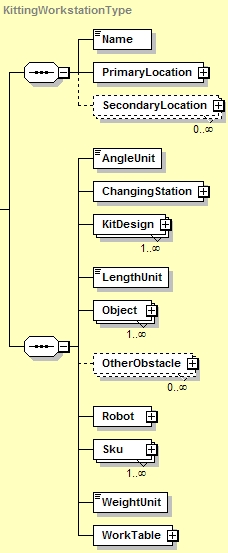
\includegraphics[width=3.166in]{images/kittingModelSmallCropped.jpg}
\caption{Kitting Workstation Model}
\label{fig:WorkstationModel}
\end{figure}

The types (i.e. classes or datatypes) of the attributes of a kitting
workstation are not shown in Figure~\ref{fig:WorkstationModel}. The
structures of several of the attributes are shown in the following figures:
\begin{itemize}
\item ChangingStation -- EndEffectorChangingStationType:
  Figure~\ref{fig:ChangingStation}
\item KitDesign -- KitDesignType: Figure~\ref{fig:KitDesign}
\item Object -- LargeBoxWithEmptyKitTraysType: Figure~\ref{fig:LBWEKT},
  LargeBoxWithKitsType: Figure~\ref{fig:LBWK}, and PartsTrayWithPartsType:
  Figure~\ref{fig:PTWP}
\item Robot -- RobotType: Figure~\ref{fig:Robot}
\item Sku -- StockKeepingUnitType: Figure~\ref{fig:SKU}
\item WorkTable -- WorkTableType: Figure~\ref{fig:WorkTable}.
\end{itemize}

The type of the Object elements in a kitting workstation is
SolidObject. That is an abstract class not intended to be
instantiated. Hence, figures \ref{fig:ChangingStation} through
\ref{fig:WorkTable} show the structures of derived classes of
SolidObject that are intended to be used for instances of the Object
attribute.

\begin{figure}[htb!]
\centering
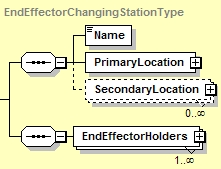
\includegraphics[width=3.166in]{images/changingStation.jpg}
\caption{Changing Station Model}
\label{fig:ChangingStation}
\end{figure}

\begin{figure}[htb!]
\centering
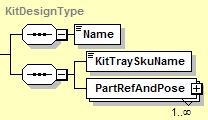
\includegraphics[width=3.1in]{images/kitDesign.jpg}
\caption{Kit Design Model}
\label{fig:KitDesign}
\end{figure}

\begin{figure}[htb!]
\centering
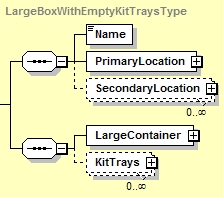
\includegraphics[width=3.1in]{images/largeBoxWithEmptyKitTrays.jpg}
\caption{Large Box With Empty Kit Trays Model}
\label{fig:LBWEKT}
\end{figure}

\begin{figure}[htb!]
\centering
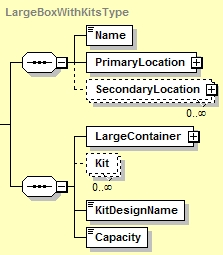
\includegraphics[width=3.1in]{images/largeBoxWithKits.jpg}
\caption{Large Box With Kits Model}
\label{fig:LBWK}
\end{figure}

\begin{figure}[htb!]
\centering
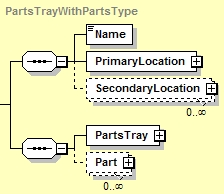
\includegraphics[width=3.1in]{images/partsTrayWithParts.jpg}
\caption{Parts Tray With Parts Model}
\label{fig:PTWP}
\end{figure}

\begin{figure}[htb!]
\centering
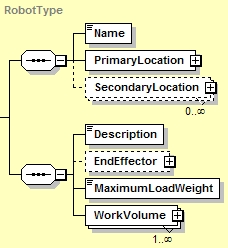
\includegraphics[width=3.166in]{images/robot.jpg}
\caption{Robot Model}
\label{fig:Robot}
\end{figure}

\begin{figure}[htb!]
\centering
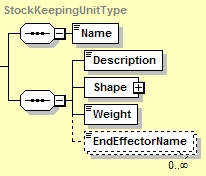
\includegraphics[width=3.166in]{images/sku.jpg}
\caption{Stock Keeping Unit Model}
\label{fig:SKU}
\end{figure}

\begin{figure}[htb!]
\centering
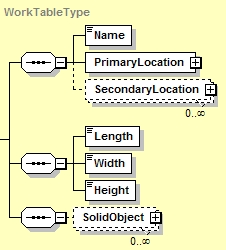
\includegraphics[width=3.166in]{images/worktable.jpg}
\caption{Work Table Model}
\label{fig:WorkTable}
\end{figure}

The robot model is simple and does not currently have any kinematics or
even any shape for the robot. It is likely that additional attributes will
be added in the future.

The kitting workstation model has been fully defined in each of two
languages: XML schema language \cite{Walmsley.2002},
\cite{XMLschemaPrimer}, \cite{XMLschemaStructures}, and Web Ontology
Language (OWL \it sic\rm) \cite{OWLoverview}, \cite{OWLprimer},
\cite{OWLspec}. Further information on the implementations may be
found in Section \ref{sect:Implementation}. 

\subsection{Robot Requirements}
As mentioned earlier, the plan format being used is a sequential list of
actions for a robot to perform. The authors devised a canonical robot
command (CRCL) language in which such lists can be written. The purpose of the
canonical robot command language is to provide generic commands that
implement the functionality of typical industrial robots without being
specific either to the language of the planning system that makes a plan or
to the language used by a robot controller that executes a plan.

It was anticipated that planning systems would plan in some language used
by automated planners and that plans made by such systems would be
translated into the canonical robot command language. It was anticipated
also that plans would be executed by a variety of robot controllers using
robot-specific languages for input programs. The authors themselves are
using a Planning Domain Definition Language (PDDL)
 planner \cite{PDDL} to generate plans in PDDL output language
and are using a ROS controller \cite{ROS} to control a robot. Those two
systems are connected using files of robot commands in CRCL. After a plan
has been generated by the PDDL planner, the plan is translated into a CRCL
file. When the plan is being executed, the CRCL commands are translated
into ROS commands.

In order to support this mode of operation, the basic robot and robotic
workcell must meet certain requirements. These include:

\begin{itemize}
\item A robot suitable for use with CRCL commands has one arm and can position
and orient the end of the arm anywhere in some work volume within some
tolerance. At each point in the work volume, the range of orientations that
can be attained may be limited.

\item The speed and acceleration of the end of the arm may be controlled.

\item A robot can attach one end effector at a time to the end of the arm at an
end effector changing station and can detach the end effector at the
changing station. The changing station itself is passive.  Attaching an end
effector is done by (1) moving the robot arm (with no end effector
attached) to an attachment position with respect to an end effector and (2)
giving a CloseToolChanger command. Detaching an end effector is done by (1)
moving the robot arm (with an end effector attached) to a detachment
position and (2) giving an OpenToolChanger command. The attachment and
detachment positions are normally at an end effector changer in the end
effector changing station.

\item All end effectors available to the robot are stored in the end effector
changing station.

\item All end effectors are assumed to be grippers.

\item All grippers have two states, open and closed. A gripper can hold an
object in the closed state and cannot hold an object in the open
state. [Additional states may be added later, such as open a certain
distance or closed with a certain force.]

\item Opening or closing any gripper mounted at the end of a robot arm is
exercised by giving a command to the robot.

\item The robot cannot simultaneously move and open or close the gripper.

\item There is always a controlled point. When no end effector is on the arm,
the controlled point is at the end of the arm. When an end effector
is mounted on the end of the arm, the controlled point is the tool
center point.

\item The robot can move the controlled point smoothly through a series of
poses from a start pose at which it is not moving to an end pose at
which it is not moving, provided that all poses are given before
motion starts. The acceleration and steady state speed of the
controlled point may be specified. The robot will do its best to
maintain the requested steady state speed but may reduce (but not
increase) speed or acceleration as necessary to allow for the dynamics
of arm motion.

\item A tolerance for the intermediate points of a smooth motion may be set.
The controlled point must pass the intermediate points within the
given tolerance (without coming back to a point after missing it by
more than the tolerance).
\end{itemize}

The CRCL includes commands for a robot controller. In normal system operation,
CRCL commands will be translated into the robot controller's native
language by the robot's plan interpreter as it works its way through a
CRCL plan. One CRCL command may be interpreted into several native
language commands.
One or more canonical robot commands may be placed on a queue and
executed (in order) when desired. Several additional assumptions are
made about the execution behavior of the robot controller. These include:

\begin{itemize}
\item If the robot controller is unable to execute a particular instance of a
canonical robot command, subsequent behavior is up to the robot
controller.

\item The pose at the end of a command is called the current pose.

\item While a plan is being executed, the robot should not move except as
directed by a canonical robot command.

\item Status of command execution is not returned by the robot controller to
the plan interpreter (or any other command generator).

\item The default coordinate system for poses used in the canonical robot commands is
the workstation coordinate system. This may be changed through the use of
a CRCL command to be either the workstation coordinate system, the
robot base coordinate system, or the tool-tip coordinate system.
\end{itemize}

The exact syntax of the CRCL commands is provided in Section \ref{sect:CRCL}.


%%%%%%%%%%%%%%%%%%%%%%%%%%%%%%%%%%%%%%%%%%%%%%%%%%%%%%%%%%%%
\section{Implementation}
\label{sect:Implementation}
The kitting workstation model has been fully defined in each of two
languages: XML schema language \cite{Walmsley.2002},
\cite{XMLschemaPrimer}, \cite{XMLschemaStructures}, and Web Ontology
Language (OWL \it sic\rm) \cite{OWLoverview}, \cite{OWLprimer},
\cite{OWLspec}. Although the two models are conceptually identical, there
are some systematic differences between the models (in addition to
differences inherent in using two different languages).

\begin{itemize}
\item The complexType names (i.e. class names) in XML schema have the
  suffix ``Type'' added which is not used in OWL. This is so that the same
  names without the suffix can be used in XML schema language as element
  names without confusion.

\item All of the XML schema complexTypes have a ``Name'' element that is
  not present in OWL. It is not needed in OWL because names are assigned as
  a matter of course when instances of classes are created.

\item The movable objects that are in the kitting workstation are
  explicitly modeled in the XML schema model but not in the OWL model.

\item Attribute names in OWL have a prefix, as described below. The
  prefixes are not used in XML schema.
\end{itemize}

\subsection{OWL Specifics}
The kitting workstation model was defined first in OWL because the IEEE RAS
Ontologies for Robotics and Automation Working Group has decided to use
OWL, and the authors are participating in the activities of that working
group. OWL allows the use of several different syntaxes. The
functional-style syntax (which is the most compact one) has been used to
write the OWL version of the kitting workstation model.

In addition to having the model defined in OWL, OWL data files describing
specific initial states and goal states were defined in OWL, also using the
functional-style syntax.  Software tools were built in C++ and Java to work with the
OWL model and data files conforming to the model.

The initial intent has been to use OWL files for presenting the initial and
goal conditions for planning problems, and the authors have implemented a
planning system that uses OWL files.

The primary tool used by the OWL community for building and checking OWL
models and data files is named Prot\'{e}g\'{e} \cite{Horridge.2011}.  Prot\'{e}g\'{e} was
used for checking the kitting model and data files as they were
built.  Prot\'{e}g\'{e} continues to be used for checking the model and data files
whenever they are changed. The layout of the hierarchy in
Figure~\ref{fig:ClassHierarchy} is identical to what may be seen in
 Prot\'{e}g\'{e}'s class hierarchy window when the kitting model is loaded.

Several difficulties of working with OWL were encountered. The primary
effect of these difficulties was to make it essentially impossible to
debug OWL files.

Defining a model in OWL is quite different from defining the same model in
other information modeling languages with which the authors are intimately
familiar: C++, EXPRESS \cite{EXPRESSmanual}, and XML schema. Three of the
major differences involve (1) the assignment of attributes in classes, (2)
OWL's ``open world'' assumption, and (3) the distinction between model
files and data files.\\

\subsubsection{Class Attributes}
In other languages, assigning a typed attribute to a class requires a
single line of code. For example, the X attribute may be put into a
cartesian point class in XML schema language with
\newline \sf $<$xs:element name=``X'' type=``xs:decimal''/$>$\rm
\newline or in C++ with
\newline \sf double X; \rm
\newline or in EXPRESS with
\newline \sf X : REAL; \rm \newline
In these other languages, the name of the attribute is local to the class.
Hence, an attribute with a given name can appear in more than one class, and
there will be no confusion.

In OWL, there is no simple method of declaring a class attribute. Instead,
a property must be declared along with properties of the property. The
following lines are used in the OWL model to say that all points and only
points have an X attribute which is a decimal number.
\newline
\newline \sf Declaration(DataProperty(hasPoint\_X))
\newline DataPropertyDomain(:hasPoint\_X :Point)
\newline DataPropertyRange(:hasPoint\_X xsd:decimal)
\newline EquivalentClasses(:Point ObjectIntersectionOf(
\newline \hspace*{0.2in}DataSomeValuesFrom(:hasPoint\_X xsd:decimal)
\newline \hspace*{0.2in}DataAllValuesFrom(:hasPoint\_X xsd:decimal))) \rm
\newline
\newline
The \sf hasPoint \rm prefix used in the property name is not an OWL
requirement. It is one of several naming conventions for OWL being used by
the authors. The prefix is both for the benefit of a human reader (to make
it obvious that this is a property of a Point) and to differentiate this X
attribute from an X attribute of some other class (call it \sf Foo\rm)
which would have the prefix \sf hasFoo \rm.

As described above, with OWL, it is necessary to make many statements in
order to build a class in a typical object-oriented style. OWL does not
assume a typical object-oriented style. It assumes the world might be more
complex than that. Hence, many OWL statements are required to produce
effects made in a few statements in other object-oriented languages. Having
to write a lot of statements is tedious but not a roadblock. A more serious
problem is that if a statement necessary to produce an object-oriented
effect is omitted, that is not an OWL error.  Prot\'{e}g\'{e} does not have an
object-oriented mode in which it will warn the user if a required statement
is missing. There are no OWL tools that will help with finding missing
statements. This is a debugging problem.

OWL was built so that it would support automated reasoning about the
relationships among properties, classes, and individuals.  Prot\'{e}g\'{e} allows
the use of several alternate automatic reasoners. In a typical
object-oriented style, there is no use for reasoning of that sort.
Everything useful to know about the relationships among properties,
classes, and individuals is already known. Hence having an automated
reasoning capability of the sort for which OWL was built is not useful
for the kitting model.\\

\subsubsection{Open World Assumption}
OWL makes an ``open world'' assumption.  In an open world, anything might
be true that is not explicitly declared false and is not inconsistent with
what has been declared true. This makes it easy for errors to go
unrecognized as such by  Prot\'{e}g\'{e} (or any other OWL tool). For example,
suppose the line \sf DataPropertyDomain(:hasPoint\_X :Point) \rm given
above is mistyped as \sf DataPropertyDomain(:hasPoint\_x :Point)\rm. When
 Prot\'{e}g\'{e} loads the file and the reasoner is started, no errors are
detected.  Prot\'{e}g\'{e} assumes that the DataPropertyDomain for \sf hasPoint\_X
\rm is unknown (tha is not an error in OWL and  Prot\'{e}g\'{e}) and that there is a new
property named \sf hasPoint\_x \rm about which the only thing known is its
DataPropertyDomain (also not an error in OWL and  Prot\'{e}g\'{e}, even though there is no
explicit DataProperty declaration for the new property). The error can be
detected by a human by studying the list provided by selecting the
DataProperties tab in  Prot\'{e}g\'{e}. Similar errors, such as mistyping the name of an individual, are
similarly accepted without error in OWL and  Prot\'{e}g\'{e}, with similar effects.
The difficulties caused by the open world assumption would not occur if
 Prot\'{e}g\'{e} had a closed world mode, but it has none.\\

\subsubsection{Model Files vs. Data Files}
While other languages have different file formats for models and
data conforming to the models, OWL does not distinguish between model files
and data files.  Prot\'{e}g\'{e} does not provide any method of specifying that a
file is a model file or a data file. The conceptual difference is simple. 
Model files describe classes and data types (and, possibly,
constraints). Data files give information about individuals (instances of
one or more classes -- often called objects). The authors have made it a
practice to distinguish OWL model files from OWL data files. An OWL data
file can inadvertently change an OWL model, a bug that is very hard to
find. That cannot happen with EXPRESS or XML schema.\\

\subsubsection{Bugs in Files}
Since humans are error-prone, and the kitting OWL files were built by
humans, the OWL files had errors of the sort mentioned above. Some of these
errors were discovered when the OWL files were processed by the tools
developed for processing them and strange results were observed. Other
errors were found when a method of generating OWL data files automatically
from XML data files was developed, as described next.

\subsection{XML Specifics}
To better explore the pros and cons of various representations,
the authors are using XML schema and XML data files in parallel with the
corresponding OWL files.\\

\subsubsection{XML Tools}
Two automated tools developed by the authors are being used: an xml schema
parser (xmlSchemaParser) and a code generator (GenXMiller).  

The xmlSchemaParser reads an XML schema file, stores it in terms of
instances of C++ classes, and reprints the schema. When the xmlSchemaParser
runs, it performs many checks on the validity of the schema that is input
to it. The xmlSchemaParser handles almost all portions of the XML schema
syntax. A few of the rarely-used bits of syntax are not implemented.

The GenXMiller reads an XML schema and writes code for reading and writing
XML data files corresponding to that schema. The code that is generated
includes C++ classes (.hh and .cc files), a parser (YACC and Lex files) and
a stand-alone parser file in C++ that uses the other files.  The executable
utility produced by compiling a stand-alone parser reads and echoes any XML
data file corresponding to the schema. The GenXMiller is still under
development and currently handles only a subset of the XML schema language. 
The GenXMiller is not a
new type of system. Several other code generators that use an XML schema
as input have been developed. Even more XML schema parsers are
available. However, having the knowledge about XML schema and XML data
files gained by developing that software and having an intimate knowledge
of the source code for it has proved very valuable in converting XML representations
to OWL representations.

The xmlSchemaParser and the GenXMiller use the same underlying parser,
which is built in YACC and Lex \cite{LexAndYACC}.

In addition to using the xmlSchemaParser and the GenXMiller, a commercial
XML tool named XMLSpy \cite{XMLSpyManual} has been used to check all XML
schemas and XML data files.\\

\subsubsection{Handling Kitting Data Files}
There is only one conceptual kitting model, but there are several kitting
data files corresponding to it. If the kitting model is used to represent
various starting and goal configurations, there
will be many more data files. Hence, the problem of generating bug-free
data files was tackled first.

An XML schema, kitting.xsd, was written by hand modeling the same
information as the OWL kitting workstation model, kittingClasses.owl. The
GenXMiller was then used to generate C++ classes and a parser for XML
kitting data files corresponding to kitting.xsd. The C++ classes that were
generated included code for printing XML kitting data
files. That code was rewritten by hand so that it prints OWL data files
rather than XML data files. The utility produced by compiling the code is
called the owlPrinter. To produce an OWL kitting data file, one writes an
XML kitting data file and runs it through the owlPrinter.

To determine that the owlPrinter works properly, it seems sufficient to
demonstrate that OWL data files generated automatically by the owlPrinter
from XML data files conforming to kitting.xsd contain exactly the same OWL
statements as are contained in manually prepared OWL data files intended to
contain the same information and conforming to kittingClasses.owl. This
demonstration was achieved as follows.

\begin{enumerate}[ (i) ]
\item Three XML data files were written manually containing the same
  information as three OWL data files. Each of the OWL files was at least
  1,100 lines (20 pages) long. Among the three there were statements of
  almost all of the types possible under the kittingClasses.owl model. It was
  decided, therefore, that successful performance for these three files
  would be an adequate test.
\item The three XML data files were run through the owlPrinter to produce
  three OWL files.
\item Since the owlPrinter has a different approach to ordering OWL
  statements as was taken in preparing OWL files manually, and a slightly
  different method of formatting statements, two small utilities were
  written to enable file comparison. The first utility, compactOwl, reads
  an OWL file and writes an OWL file containing the same statements but
  with blank lines and comments removed, and with each statement on a
  single line. For each pair of matching OWL files (manually written and
  automatically generated), compactOwl was used to generate a corresponding
  pair of compacted OWL files. The second utility, compareOwl, reads each
  of a pair of OWL files, alphabetizes the statements from each of them on
  two saved lists, and then goes through the two lists checking that the
  n$^{th}$ line of one list is identical to the n$^{th}$ line of the other list.
  CompareOwl was used to compare each of the three sets of pairs of
  compacted files.
\item While the tests just described were being made, changes were made to
  correct errors in the manually written XML and OWL data files being
  tested and in the code for the owlPrinter. The tests revealed errors in
  all three types of files.
\end{enumerate}

After the testing just described was complete, using the owlPrinter,
another OWL data file was prepared from a manually written XML data file
for which there was no manually written OWL counterpart. The automatically
generated OWL data file was checked in  Prot\'{e}g\'{e} and no errors were reported.

OWL data files
may now be prepared with much less likelihood of human error for the following
reasons.
\begin{itemize}

\item Property names and names of individuals will not be misspelled.

\item Statements will not be accidentally omitted.

\item Validity checks made in the kittingParser and XMLSpy will do a
  better job of detecting errors in XML data files. For example, required
  attributes that are missing will be detected.

\end{itemize}

\subsubsection{Handling the Kitting Model}
As described above, the equivalent model files kitting.xsd and
kittingClasses.owl were both prepared manually. If changes to the kitting
model are made, it will be necessary to change both of those files and the
code for the owlPrinter. It would be good to have kitting.xsd as the
primary source file for the model and to generate kittingClasses.owl
automatically from it. The authors believe this is possible and have
started working on it. The work is not yet complete, but no roadblocks are
anticipated. The approach being using is to modify the printer code in the
xmlSchemaParser so that it prints an OWL class file rather than an XML
schema file.

It would also be desirable to be able to modify the owlPrinter
automatically if the kitting model is changed. Doing that is a
substantially more difficult task than the other two automatic conversions,
and the authors are not planning to attempt it. The approach would be to
modify the GenXMiller so that the code it generates automatically would
read XML data files and automatically generate OWL data files.

\subsection{Robot Control Language}
\label{sect:Implementation.CRCL}
It is desirable to have numerous commercial robot systems be able to 
immediately execute the plan for the series of actions required to transition from the initial state
to the goal state of the kitting problem. However, there is currently no
accepted standard robot programming language. For this reason, the authors
have put together a ``canonical robot control language" (CRCL) that attempts to be
a lowest common denominator of robot programing languages. It is anticipated
that kitting plans can be translated into  CRCL command sets which may then be
evaluated by standardized metric software. The CRCL command sets may then
be translated into a specific robot platform's language.

The syntax of commands is given below using C++ syntax. The command
name is given followed by the command arguments (if any) in parentheses,
including the types of the arguments.
Note that the robot cannot be commanded by canonical robot commands in
terms of its joint angles (or distances).

Three of the CRCL commands use the Pose structure. The Pose structure gives
the location and orientation of the coordinate system of the controlled
object in the units of the current operating coordinate system. 
The controlled object is the gripper if the robot has one attached
or the outermost component of the robot arm if not.  The location is
specified by the point in current operating coordinates at which the
origin of the coordinate system of the controlled object lies. The point is
described by giving its X, Y, and Z values. The orientation of the
controlled object is specified by giving the I, J, and K components in
current operating coordinates of the Z and X axes of the coordinate
system of the controlled object. 

The complete list of CRCL commands follows.\\

\begin{itemize}

\item \sf CloseGripper() \rm -- Close the gripper.\\

\item \sf CloseToolChanger() \rm -- Close the tool changer on the robot so
  that it attaches to a tool. The robot must be in an appropriate position
  with respect to the tool for the changer mechanism on the robot to attach
  to the tool.\\

\item \sf Dwell (double time) \rm -- Stay motionless for the given amount
  of \sf time \rm in seconds.\\

\item \sf EndCanon(int reason) \rm -- Do whatever is necessary to stop
  executing canonical robot commands. No specific action is required. The
  robot controller should not execute any canonical robot command except
  \sf InitCanon \rm after executing \sf EndCanon \rm and should signal an
  error if it is given one.  This command will normally be given when
  execution of a plan is complete.  It may also be given if the plan
  interpreter detects an error in the plan or is unable to proceed for any
  other reason. A value of 0 for \sf reason \rm indicates that execution of
  a plan has completed successfully.  A positive value of reason indicates
  not.\\

\item \sf InitCanon() \rm -- Do whatever is necessary to get ready to
move. Length units, angle units, and operating coordinate system are 
set to the default units. This command
will normally be given when the plan interpreter opens a plan to be
executed.\\

\item \sf Message (string message) \rm -- Display the given \sf message \rm
  on the operator console.\\

\item \sf MoveStraightTo(Pose * pose) \rm -- Move the controlled point in a
  straight line from the current pose to the given \sf pose\rm, and stop
  there.\\

\item \sf MoveThroughTo(Pose ** poses, int numPoses) \rm -- Move the
  controlled point along a trajectory passing near all but the last of the
  given \sf poses\rm, and stop at the last of the given \sf poses\rm.
  The \sf numPoses \rm gives the number of poses.\\

\item \sf MoveTo(Pose * pose) \rm -- Move the controlled point along any
  convenient trajectory from the current pose to the given \sf pose\rm,
  and stop there.\\

\item \sf OpenGripper() \rm -- Open the gripper.\\

\item \sf OpenToolChanger() \rm -- Open the tool changer on the robot so
  that it releases the end effector.  This is normally done after the end
  effector attached to the robot has been moved into an end effector
  changer.\\

\item \sf SetAbsoluteAcceleration(double acceleration) \rm -- Set the
  acceleration for the controlled point to the given value in length units
  per second per second.\\

\item \sf SetAbsoluteSpeed(double speed) \rm -- Set the speed for the
  controlled point to the given value in length units per second.\\

\item \sf SetAngleUnits(string UnitName) \rm -- Set angle units to the unit
  named by the \sf UnitName\rm.  The \sf UnitName \rm must be one of
  ``degree'' or ``radian''. All commands that use angle units (for
  orientation or orientation tolerance) are in terms of those angle
  units. Existing values for orientation are converted automatically to the
  equivalent value in new angle units.  The default angle unit is
  ``degree''.\\

\item \sf SetCoordinateFrame(string CoordSystem) \rm -- Set the
operating coordinate system to the system referred to by
\sf CoordSystem\rm. The \sf CoordSystem\rm must be one of
``Workstation", ``RobotBase", or ``ToolTip".

\item \sf SetEndAngleTolerance(double tolerance) \rm -- Set the tolerance
  for the orientation of the end of the arm (whenever there is no gripper
  there) or of the gripper (whenever a gripper is on the end of the arm) to
  the given value in current angle units.\\

\item \sf SetEndPointTolerance(double tolerance) \rm -- Set the tolerance
  for the position of the end of the arm (whenever there is no gripper
  there) or of the tool centre point (whenever a gripper is on the end of
  the arm) to the given value in current length units.\\

\item \sf SetIntermediatePointTolerance(double tolerance) \rm -- Set the
  tolerance for smooth motion near intermediate points to the given value
  in current length units.\\

\item \sf SetLengthUnits(string UnitName) \rm -- Set length units to the
  unit named by the \sf UnitName\rm.  The \sf UnitName \rm must be one of
  ``inch'', ``mm'' or ``meter''. All commands that use length units (for
  location, tolerance, speed, and acceleration) are in terms of those
  length units. Existing values for speed, position, acceleration, etc. are
  converted automatically to the equivalent value in new length units. The
  default length unit is millimeters, ``mm''.\\

\item \sf SetRelativeAcceleration(double percent) \rm -- Set the
  acceleration for the controlled point to the given percentage of the
  robot's maximum acceleration.\\

\item \sf SetRelativeSpeed(double percent) \rm -- Set the speed for the
  controlled point to the given percentage of the robot's maximum speed.\\

The next two items do not seem to really belong here. I understand why
Teddy put them here (he needed the commands), but they seem too specific.
Any suggestions on how to make them more general? I was thinking of a
general ``StartRobotSubSystem(string name, string parameter)".
\item \sf StartObjectScan(string name) \rm -- Activate the object sensor,
  if it isn't already activated, and add the given \sf name \rm to the list of
  parts being searched for.\\

\item \sf StopObjectScan() \rm -- Deactivate the object sensor.\\

\item \sf StopMotion(integer isEmergency) \rm -- Stop the robot motion. If
  \sf isEmergency \rm is not 0, then stop as soon as possible regardless of
  damage to the system. If \sf isEmergency \rm is 0 then come to a graceful
  stop.\\

\end{itemize}

A file format for representing CRCL commands has been devised.
Figure~\ref{fig:KittingPlan} shows an example of a file prepared using this
format. A C++ class model of CRCL commands has been built, and a parser has
been built in C++ for reading CRCL files and populating
CRCL class instances.

\subsection{Plan Model}
The kitting system presented in this document relies on a \textit{direct} model of execution where the executor directly performs the activities specified in the plan. Figure~\ref{fig:executor} depicts the executor process for the kitting domain where ellipses represent files, regular rectangles are used to define processes, and rounded rectangles illustrate tools. The red dashed box contains the processes part of the executor. The components in Figure~\ref{fig:executor} are described below:

\begin{enumerate}
\item PDDL domain and problem files are generated from the IEEE RAS  Ontologies for Robotics and Automation Working Group's ontology and are used by a planner to generate a plan file.
The plan file contains a sequence of actions that can be executed from the initial state and that leads to a goal state. The actions present in the plan file are originally defined in the PDDL domain file. The initial and goal states are defined in the PDDL problem file.

\item The interpreter takes the plan file as input and builds the corresponding CRCL file. The knowledge representation is required to locate objects in the environment. Table~\ref{tab:takepart} shows an example of CRCL commands generated for the PDDL action \stvar{take-part(part\_b\_1)}. Please note that the PDDL action \stvar{take-part} developed for the current kitting domain has more than one parameter. All the parameters are not relevant for the example depicted in Table~\ref{tab:takepart} and the number of parameters has been subsequently reduced for simplicity.

\begin{table}[h!]
\centering

    \begin{tabular}{l}
    \stvar{take-part(part\_b\_1)}\\
    \hline
    \hline
  \texttt{\scriptsize{Message (``take part part\_b\_1")}}\\
  \texttt{\scriptsize{MoveTo(\{\{-0.03, 1.62, -0.25\}, \{0, 0, 1\}, \{1, 0, 0\}\})}}\\
  \texttt{\scriptsize{Dwell (0.05)}}\\
  \texttt{\scriptsize{MoveTo(\{\{-0.03, 1.62, 0.1325\}, \{0, 0, 1\}, \{1, 0, 0\}\})}} \\
  \texttt{\scriptsize{CloseGripper ()}} \\
  \texttt{\scriptsize{MoveTo(\{\{-0.03, 1.62, -0.25\}, \{0, 0, 1\}, \{1, 0, 0\}\})}}\\
  \texttt{\scriptsize{Dwell (0.05)}}\\
  \hline
  \end{tabular}
\caption{An example of CRCL commands for a PDDL action.}
  \label{tab:takepart}
\end{table}

\item The CRCL file is used by the controller in order to create ROS commands.

\item The ROS commands are used by the ROS software controller for a robotic arm to initiate actual execution of actions.

\end{enumerate}

\begin{figure}[ht!]
\begin{center}
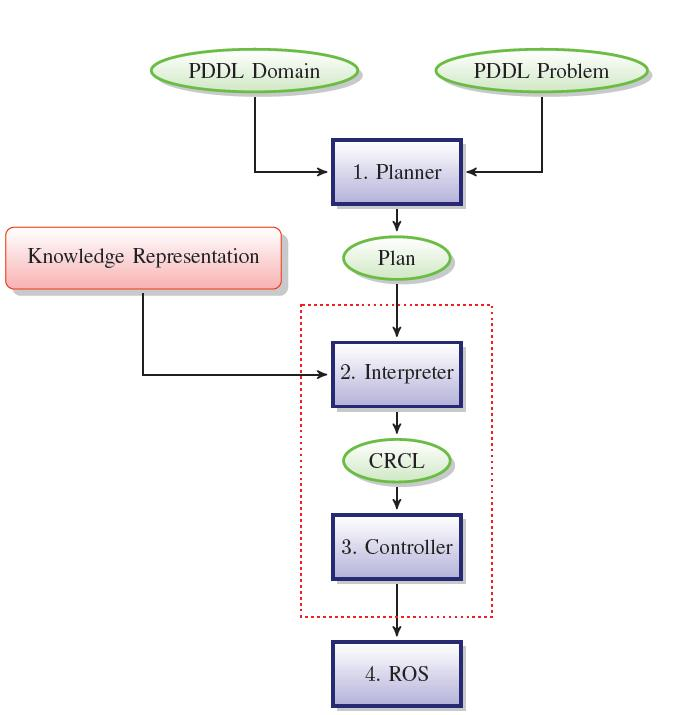
\includegraphics[width=8cm]{images/executordiag.jpg}
\caption{The executor process.}
\label{fig:executor}
\end{center}
\end{figure}



%%%%%%%%%%%%%%%%%%%%%%%%%%%%%%%%%%%%%%%%%%%%%%%%%%%%%%%%%%%%
\section{Canonical Robot Control Language}
\label{sect:CRCL}

It is desirable that numerous commercial robot systems be able to 
immediately execute the plan for the series of actions required to transition from the initial state
to the goal state of the kitting problem. However, there is currently no
accepted standard robot programming language. For this reason, the authors
have developed a ``canonical robot control language" (CRCL) that attempts to be
a lowest common denominator of robot programing languages. It is anticipated
that kitting plans can be translated into  CRCL command sets which may then be
evaluated by standardized metric software. The CRCL command sets may then
be translated into a specific robot platform's language.

The syntax of commands is given below using C++ syntax. The command
name is given followed by the command arguments (if any) in parentheses,
including the types of the arguments.
Note that the robot cannot be commanded by canonical robot commands in
terms of its joint angles (or distances).

Three of the CRCL commands use the Pose structure. The Pose structure gives
the location and orientation of the coordinate system of the controlled
object in the units of the current operating coordinate system. 
The controlled object is the gripper if the robot has one attached
or the outermost component of the robot arm if not.  The location is
specified by the point in current operating coordinates at which the
origin of the coordinate system of the controlled object lies. The point is
described by giving its X, Y, and Z values. The orientation of the
controlled object is specified by giving the I, J, and K components in
current operating coordinates of the Z and X axes of the coordinate
system of the controlled object. 

The complete list of CRCL commands follows.

\begin{itemize}

\item \sf CloseGripper() \rm -- close the gripper.\\

\item \sf CloseToolChanger() \rm -- close the tool changer on the robot so
  that it attaches to a tool. The robot must be in an appropriate position
  with respect to the tool for the changer mechanism on the robot to attach
  to the tool.\\

\item \sf Dwell (double time) \rm -- stay motionless for the given amount
  of \sf time \rm in seconds.\\

\item \sf EndCanon(int reason) \rm -- do whatever is necessary to stop
  executing canonical robot commands. No specific action is required. The
  robot controller should not execute any canonical robot command except
  \sf InitCanon \rm after executing \sf EndCanon \rm and should signal an
  error if it is given one.  This command will normally be given when
  execution of a plan is complete.  It may also be given if the plan
  interpreter detects an error in the plan or is unable to proceed for any
  other reason. A value of 0 for \sf reason \rm indicates that execution of
  a plan has completed successfully.  A positive value of reason indicates
  not.\\

\item \sf InitCanon() \rm -- do whatever is necessary to get ready to
move. Length units, angle units, and operating coordinate system are 
set to the default units. This command
will normally be given when the plan interpreter opens a plan to be
executed.\\

\item \sf Message (string message) \rm -- display the given \sf message \rm
  on the operator console.\\

\item \sf MoveStraightTo(Pose * pose) \rm -- move the controlled point in a
  straight line from the current pose to the given \sf pose\rm, and stop
  there.\\

\item \sf MoveThroughTo(Pose ** poses, int numPoses) \rm -- move the
  controlled point along a trajectory passing near all but the last of the
  given \sf poses\rm, and stop at the last of the given \sf poses\rm.
  The \sf numPoses \rm gives the number of poses.\\

\item \sf MoveTo(Pose * pose) \rm -- move the controlled point along any
  convenient trajectory from the current pose to the given \sf pose\rm,
  and stop there.\\

\item \sf OpenGripper() \rm -- open the gripper.\\

\item \sf OpenToolChanger() \rm -- open the tool changer on the robot so
  that it releases the end effector.  This is normally done after the end
  effector attached to the robot has been moved into an end effector
  changer.\\

\item \sf SetAbsoluteAcceleration(double acceleration) \rm -- set the
  acceleration for the controlled point to the given value in length units
  per second per second.\\

\item \sf SetAbsoluteSpeed(double speed) \rm -- set the speed for the
  controlled point to the given value in length units per second.\\

\item \sf SetAngleUnits(string UnitName) \rm -- set angle units to the unit
  named by the \sf UnitName\rm.  The \sf UnitName \rm must be one of
  ``degree'' or ``radian''. All commands that use angle units (for
  orientation or orientation tolerance) are in terms of those angle
  units. Existing values for orientation are converted automatically to the
  equivalent value in new angle units.  The default angle unit is
  ``degree''.\\

\item \sf SetCoordinateFrame(string CoordSystem) \rm -- set the
operating coordinate system to the system referred to by
\sf CoordSystem\rm. The \sf CoordSystem \rm must be one of
``Workstation", ``RobotBase", or ``ToolTip".\\

\item \sf SetEndAngleTolerance(double tolerance) \rm -- set the tolerance
  for the orientation of the end of the arm (whenever there is no gripper
  there) or of the gripper (whenever a gripper is on the end of the arm) to
  the given value in current angle units. This applies to the X-axis direction
and the Z-axis direction.\\

\item \sf SetEndPointTolerance(double tolerance) \rm -- set the tolerance
  for the position of the end of the arm (whenever there is no gripper
  there) or of the tool centre point (whenever a gripper is on the end of
  the arm) to the given value in current length units.\\

\item \sf SetIntermediatePointTolerance(double tolerance) \rm -- set the
  tolerance for smooth motion near intermediate points to the given value
  in current length units.\\

\item \sf SetLengthUnits(string UnitName) \rm -- set length units to the
  unit named by the \sf UnitName\rm.  The \sf UnitName \rm must be one of
  ``inch'', ``mm'' or ``meter''. All commands that use length units (for
  location, tolerance, speed, and acceleration) are in terms of those
  length units. Existing values for speed, position, acceleration, etc. are
  converted automatically to the equivalent value in new length units. The
  default length unit is millimeters, ``mm''.\\

\item \sf SetRelativeAcceleration(double percent) \rm -- set the
  acceleration for the controlled point to the given percentage of the
  robot's maximum acceleration.\\

\item \sf SetRelativeSpeed(double percent) \rm -- set the speed for the
  controlled point to the given percentage of the robot's maximum speed.\\

%\vspace{.1in} \sf The next two items do not seem to really belong here. I understand why
%Teddy put them here (he needed the commands), but they seem too specific.
%Any suggestions on how to make them more general? I was thinking of a
%general ``StartRobotSubSystem(string name, string parameter)". \rm \\ \\
%\item \sf StartObjectScan(string name) \rm -- Activate the object sensor,
%  if it isn't already activated, and add the given \sf name \rm to the list of
%  parts being searched for.\\
%
%\item \sf StopObjectScan() \rm -- deactivate the object sensor.\\

\item \sf StopMotion(integer isEmergency) \rm -- stop the robot motion. If
  \sf isEmergency \rm is not 0, then stop as soon as possible regardless of
  damage to the system. If \sf isEmergency \rm is 0 then come to a graceful
  stop.\\

\end{itemize}

A file format for representing CRCL commands has been devised.
Figure~\ref{fig:KittingPlan} shows an example of a file prepared using this
format. A C++ class model of CRCL commands has been built, and a parser has
been built in C++ for reading CRCL files and populating
CRCL class instances.

\subsection{Plan Model}
The kitting system presented in this document relies on a \textit{direct} model of execution where the executor directly performs the activities specified in the plan. Figure~\ref{fig:executor} depicts the executor process for the kitting domain where ellipses represent files, regular rectangles are used to define processes, and rounded rectangles illustrate tools. The red dashed box contains the processes part of the executor. The components in Figure~\ref{fig:executor} are described below:

\begin{enumerate}
\item PDDL domain and problem files are currently generated by hand from the IEEE RAS  Ontologies for Robotics and Automation Working Group's
OWL-based knowledge representation
and are used by an open source planner from Coles et al. \cite{Coles.ICAPS.2010} to automatically generate a plan file. In the near future, these files will be automatically generated.
The plan file contains a sequence of actions that can be executed from the initial state and that lead to a goal state. The actions present in the plan file are originally defined in the PDDL domain file. The initial and goal states are defined in the PDDL problem file.

\item The interpreter takes the plan file as input and builds the corresponding CRCL file. Real time information on the environment is required in order to fill in information required by the CRCL on
object locations. Since both the OWL and XML implementations of the knowledge representation are file based, real time information proved to be problematic. In order to solve this problem,
an automatically generated MySQL database \cite{MySQL} has been introduced as part of the knowledge representation. More details on this database are provided in Section \ref{sect:MySQL}.
Table~\ref{tab:takepart} shows an example of CRCL commands generated for the PDDL action \stvar{take-part(part\_b\_1)}. Please note that the PDDL action \stvar{take-part} developed for the current kitting domain has more than one parameter. Not all the parameters are relevant for the example depicted in Table~\ref{tab:takepart} and the number of parameters has been  reduced for simplicity. In this example,
the locations of the \lq\lq{}MoveTo\rq\rq{} commands would come from the MySQL database.

\begin{table}[h!]
\centering

    \begin{tabular}{l}
    \stvar{take-part(part\_b\_1)}\\
    \hline
    \hline
  \texttt{\scriptsize{Message (``take part part\_b\_1")}}\\
  \texttt{\scriptsize{MoveTo(\{\{-0.03, 1.62, -0.25\}, \{0, 0, 1\}, \{1, 0, 0\}\})}}\\
  \texttt{\scriptsize{Dwell (0.05)}}\\
  \texttt{\scriptsize{MoveTo(\{\{-0.03, 1.62, 0.1325\}, \{0, 0, 1\}, \{1, 0, 0\}\})}} \\
  \texttt{\scriptsize{CloseGripper ()}} \\
  \texttt{\scriptsize{MoveTo(\{\{-0.03, 1.62, -0.25\}, \{0, 0, 1\}, \{1, 0, 0\}\})}}\\
  \texttt{\scriptsize{Dwell (0.05)}}\\
  \hline
  \end{tabular}
\caption{An example of CRCL commands for a PDDL action}
  \label{tab:takepart}
\end{table}

\item The CRCL file is used by the controller to create ROS commands.

\item The ROS commands are used by the ROS software controller for a robotic arm to initiate actual execution of actions.

\end{enumerate}

\begin{figure}[ht!]
\begin{center}
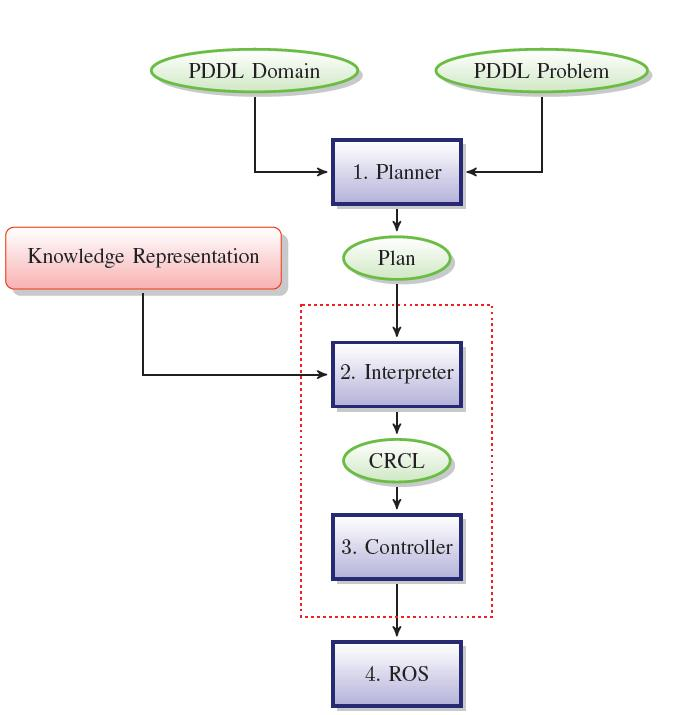
\includegraphics[width=8cm]{images/executordiag.jpg}
\caption{The executor process}
\label{fig:executor}
\end{center}
\end{figure}



%%%%%%%%%%%%%%%%%%%%%%%%%%%%%%%%%%%%%%%%%%%%%%%%%%%%%%%%%%%%
\section{MySQL Database for Kitting}
\label{sect:MySQL}
While the knowledge representation presented in this paper provides the \lq\lq{}slots\rq\rq{} necessary for representing dynamic information, the
static file structure makes the utilization of these slots awkward. It is desirable to be able to represent the dynamic information in a dynamic database.
For this reason, the authors have developed a technique for automatically generating tables for storing,  and access functions
for obtaining, the data from the ontology in a MySQL database.

Reading data from and to the MySQL database instead of the ontology file offers the community easy access to a live data structure. Furthermore, it is more practical to modify the information stored in a database than if it was stored in an ontology, which in some cases, requires the deletion and re-creation of the whole file. A literature review reveals many efforts and methodologies that have been designed to produce SQL databases from ontologies. Our effort builds upon the work of Astrova et al.\cite{Astrova2007}. 

In addition to generating and filling the database tables, the authors have created tools that automatically generate a set of C++ classes for reading and writing
information to the kitting MySQL database. The choice of C++ was a team preference and we believe that other object-oriented languages could have been used in this project.

The Generator tool is a graphical user interface developed in Java, allowing the user to store data from OWL files into a MySQL database. This tool also permits the user to query the database using the C++ function calls. The tool Generator is composed of the following functionalities:
\begin{enumerate}
 \item Convert OWL documents into SQL syntaxes (OWL to SQL).
 \item Translate SQL syntaxes to OWL language in order to modify an OWL document (SQL to OWL).
 \item Convert the OWL language into C++ classes (OWL to C++).
\end{enumerate}

To date, only steps 1. and 3. have been implemented and will be covered in this document.
In order to generate the SQL database and C++ classes, the OWL object model must be mapped to the C++ object model and the relational SQL model. 
To quote the OWL 2 Web Ontology website~\cite{OWLspec}, ``Entities are the fundamental building blocks of OWL 2 ontologies, 
and they define the vocabulary --the named terms-- of an ontology. In logic, the set of entities is usually said to constitute the 
signature of an ontology''. Therefore, the notions of single-valued and multi-valued properties as well as the inheritance must be 
mapped from the ontology to the SQL database and C++ classes. The mapping from OWL proceeds as follows:
\begin{itemize}
\item Data properties: In an ontology, data properties link an individual to a data value. Single-valued data properties are mapped into a SQL table entry or C++ class
variable with the corresponding type of the original property. For example, in the ontology a robot has a single-valued data 
property \texttt{hasRobot\_Description}, represented in the
SQL database as a \texttt{varchar} and in the corresponding C++ class as \texttt{std:string}. 
Multi-valued data properties are mapped from the ontology into the SQL database as a table and into the C++ class as a \texttt{std:vector} with the corresponding
type of the original property. For example,
in the ontology a stock keeping unit has a multi-valued
data property \texttt{hasSku\_EndEffectorRefs}. This maps to a SQL table containing \texttt{varchar} entries and the C++
\texttt{std::vector\textless std::string\textgreater} in the corresponding C++ class.

\item Object property: In an ontology, object properties link one individual to another individual. 
The single-valued object properties are mapped to a SQL table entry or C++ class
variable. Their type is a pointer to the range of the object properties. For example, in the ontology a solid object has the object property \texttt{hasRobot\_Description} 
linking it to a physical location. In the SQL database, we use the a foreign key to link the two entries. In the C++ classes, this is represented by a reference to a physical location: \texttt{PhysicalLocation* hasSolidObject\_PrimaryLocation}.
Multi-valued object properties are mapped from the ontology into the SQL database as a table and into the C++ class as a \texttt{std:vector} of pointers referencing objects of the range of the property.  For example, a solid object also has a list of secondary locations corresponding to a multi-valued object property in the ontology: {\scriptsize\texttt{std::vector\\ \textless PhysicalLocation*\textgreater hasSolidObject\_SecondaryLocation}}.
\end{itemize}

\subsection{MySQL Database Generation}\label{ss:ontology2db}
\begin{figure}[h!t!]
\centering
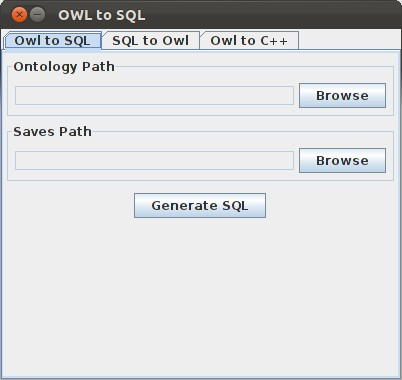
\includegraphics[width=8.5cm]{images/OWLtoSQL001.jpeg}
\caption{Owl to SQL tab.}
\label{fig:owl2sql}
\end{figure}

This section provides basic information on the Generator Java tool. Specific information on the tools usage is included with the tool in its manual.
Converting an OWL ontology to SQL script files is easily performed using the \texttt{Owl to SQL} tab  (see Figure~\ref{fig:owl2sql}). The required fields are:

\begin{itemize}
 \item Ontology Path: The OWL file to be converted. Note that all \texttt{Import} statements in this file must use absolute paths.
 \item Saves Path: The directory where you want to save the SQL files.
\end{itemize}

Clicking on the ``Generate SQL'' will generate the SQL script files. Two files will be created by the tool:
\begin{itemize}
\item The file used to create tables in the database: \texttt{<inputfile>.owlCreateTable.sql} 
\item The file used to populate the database tables: \texttt{<inputfile>.owlInsertInto.sql}. 
\end{itemize}
These files may then be used with the SQL command line interface to create and populate the database.

\subsection{C++ Class Generation and Usage}
As previously mentioned, the C++ classes are automatically generated by the Generator tool. In addition to the class structure, 
Data Access Objects (DAO) that are needed to interact with the MySQL database are generated. 
To map the MySQL database and indirectly the ontology to C++ classes, both the C++ classes and
the DAO must be generated.

The C++ class files (.cpp) and header files (.h) are generated in a two step process.
The first step does not depend on the content of the ontology, it only initializes the specific objects related to the MySQL connector driver
(see Figure~\ref{fig:headerclass}).

The second step generates all the C++ headers and class files relative to our ontology. 
All of the \texttt{include} statements  are made directly in the C++ class files, and only forward declarations are performed in the headers. 
This resolves problems associated with circular includes or multiple includes. All of the classes include the following methods:
\begin{itemize}
\item \texttt{get<private field>} - Method for getting a private field.
\item \texttt{set<private field>} - Method for setting a private field.
\item \texttt{explode} - Method that splits a string into a vector around matches of a given regular expression. 
\item \texttt{copy} -  Method that takes a C++ map as input and copy the values from the map into the instance.
\item \texttt{get} - Method that reads data from the MySQL database.
\item \texttt{set} - Method that writes data to the MySQL database.
\end{itemize}

\begin{figure}[t!h!]
\begin{minipage}{.45\paperwidth}
\begin{mylisting}
\begin{Verbatim}[commandchars=\\\{\},fontsize=\scriptsize, numbersep=2pt]
\textbf{#ifndef} PARTSBIN_H_
\textbf{#define} PARTSBIN_H_
\textbf{#include} <cstdlib>
\textbf{#include} <iostream>
\textbf{#include} <map>
\textbf{#include} <string>
\textbf{#include} <vector>
\textbf{#include} <sstream>

\textbf{#include} "BoxyObject.h"
\textbf{class} DAO;
\textbf{class} PartsBin: \textbf{public} BoxyObject \{
    \textbf{private}:
        std::string hasBin_PartQuantity;
        std::string hasBin_PartSkuRef;
        \textbf{int} PartsBinID;
        DAO* dao;
    \textbf{public}:
        PartsBin(std::string name);
        ~PartsBin();
        \textbf{void} get(\textbf{int} id);
        \textbf{void} get(std::string name);
        \textbf{void} set(\textbf{int} id, PartsBin* obj);
        \textbf{void} set(std::string name);
        std::string gethasBin_PartQuantity();
        \textbf{void} sethasBin_PartQuantity(
            std::string _hasBin_PartQuantity);
        std::string gethasBin_PartSkuRef();
        \textbf{void} sethasBin_PartSkuRef(
            std::string _hasBin_PartSkuRef);
        \textbf{int} getPartsBinID();
        DAO* getdao();
        \textbf{void} setdao(DAO* _dao);
        \textbf{void} copy(std::map<std::string,
            std::string> object);
        std::vector<std::string> Explode(
            \textbf{const} std::string & str, \textbf{char} separator);
\};
\textbf{#endif} /* PARTSBIN_H_ */
\end{Verbatim}
\end{mylisting}
\end{minipage}
\caption{Header of a generated class.}
\label{fig:headerclass}
\end{figure}



%\lstset{frame=single, language=C++, caption=Header of a generated class, label=Header of a generated class,
%captionpos=b}
%\begin{lstlisting}
%#ifndef PARTSBIN_H_
%#define PARTSBIN_H_
%#include <cstdlib>
%#include <iostream>
%#include <map>
%#include <string>
%#include <vector>
%#include <sstream>
%
%#include "BoxyObject.h"
%class DAO;
%class PartsBin: public BoxyObject {
%private:
%	std::string hasBin_PartQuantity;
%	std::string hasBin_PartSkuRef;
%	int PartsBinID;
%	DAO* dao;
%public:
%	PartsBin(std::string name);
%	~PartsBin();
%	void get(int id);
%	void get(std::string name);
%	void set(int id, PartsBin* obj);
%	void set(std::string name);
%	std::string gethasBin_PartQuantity();
%	void sethasBin_PartQuantity(
%		std::string _hasBin_PartQuantity);
%	std::string gethasBin_PartSkuRef();
%	void sethasBin_PartSkuRef(
%		std::string _hasBin_PartSkuRef);
%	int getPartsBinID();
%	DAO* getdao();
%	void setdao(DAO* _dao);
%	void copy(std::map<std::string, std::string> object);
%	std::vector<std::string> Explode(
%		  const std::string & str, char separator);
%};
%#endif /* PARTSBIN_H_ */
%\end{lstlisting}



The actual data access is provided through the use of a data access object (DAO).
DAOs provide an abstract interface to some type of database or other persistence
mechanism. DAOs map application calls to the database or persistence mechanism, 
thus providing some specific data operations without exposing
details of the database. The use of the DAO separates the data accesses that the application needs from how these needs can be satisfied with a specific
Database Management System (DBMS), database schema, etc. 
The different methods of the DAO are the same for any ontology. 
The concern here is not about the data, but only about the way to retrieve or store it. Only the four vectors filled by the
private \texttt{fillGetSqlQueries} method differ from one 
auto-generated C++ file to another file.

When the DAO is generated, four vectors are built as follows (shown in Figure \ref{fig:headerdao}):

\begin{itemize}
\item line \textcolor{BrickRed}{17} : A structure with the SQL query to select the content of the tables relative to an entity, the table relative to the entity itself and the ones relative to its super classes.
\item line \textcolor{BrickRed}{18} : A structure with the SQL query to select the multi-valued attributes (multi-valued data) for a given entity.
\item line \textcolor{BrickRed}{19} : A structure with the names of the tables linked to this entity in the ontology.
\item line \textcolor{BrickRed}{20} : A structure with the names of the association tables linked to an object.
\end{itemize}

With these four structures, one is able to read (\texttt{get} method) and write (\texttt{set} method) data from and to the MySQL database. The \texttt{get} method fills 
a C++ map and gets the object itself while the \texttt{copy} method handles the data. The \texttt{set} method is called with a C++ map containing the values of the 
different attributes as input and writes these values into the MySQL database.


\begin{figure}[t!h!]
\begin{minipage}{.45\paperwidth}
\begin{mylisting}
\begin{Verbatim}[commandchars=\\\{\},fontsize=\scriptsize, numbers=left, numbersep=2pt]
\textbf{#ifndef} DAO_H_
\textbf{#define} DAO_H_
\textbf{#include} <cstdlib>
\textbf{#include} <iostream>
\textbf{#include} <map>
\textbf{#include} <vector>
\textbf{#include} <sstream>

\textbf{#include} "Connection.h"
\textbf{class} DAO \{
    \textbf{private}:
      std::vector<std::string> className;
      Connection* connection;
      std::vector<std::string> nameDone;
      std::map<std::string, std::string> map;
      std::string path; std::string pathmulti;
      \textbf{static} std::map<std::string, std::string>
        getSqlQueriesDataSingle;
      \textbf{static} std::map<std::string, 
			std::vector<std::string>>
			getSqlQueriesDataMulti;
      \textbf{static} std::map<std::string, 
			std::vector<std::string>>
			getSqlQueriesObjectSingle;
      \textbf{static} std::map<std::string, 
			std::vector<std::string>>
			getSqlQueriesObjectMulti;
      \textbf{static} std::map<std::string, 
			std::vector<std::string>>
			setSqlQueries;
      \textbf{static} std::map<std::string, 
			std::vector<std::string>>
			updateSqlQueries;
      \textbf{void} fillGetSqlQueries();
    \textbf{public}:
      DAO(std::string name); ~DAO();
      std::vector<std::string> getclassName();
      \textbf{void} setclassName(
		std::vector<std::string> _className);
      Connection* getconnection();
      \textbf{void} setconnection(Connection* _connection);
      std::map<std::string,std::string> 
      	get(std::string name);
      \textbf{void} set(std::map<std::string, std::string> data);
      std::vector<std::string> Explode(
		\textbf{const} std::string & str,
      \textbf{char separator});
\};
\textbf{#endif} /* DAO_H_ */
\end{Verbatim}
\end{mylisting}
\end{minipage}
\caption{Header of the DAO class.}
\label{fig:headerdao}
\end{figure}


%\lstset{frame=single, language=C++, caption=Header of our DAO class, label=Header of our DAO class,
%captionpos=b}
%\begin{lstlisting}
%#ifndef DAO_H_
%#define DAO_H_
%#include <cstdlib>
%#include <iostream>
%#include <map>
%#include <vector>
%#include <sstream>
%#include "Connection.h"
%class DAO {
%private:
%	std::vector<std::string> className;
%	Connection* connection;
%	std::vector<std::string> nameDone;
%	std::map<std::string, std::string> map;
%	std::string path; std::string pathmulti;
%	static std::map<std::string, std::string>
%				  getSqlQueriesDataSingle;
%	static std::map<std::string, std::vector<std::string> >
%			getSqlQueriesDataMulti;
%	static std::map<std::string, std::vector<std::string> >
%			getSqlQueriesObjectSingle;
%	static std::map<std::string, std::vector<std::string> >
%			getSqlQueriesObjectMulti;
%	static std::map<std::string, std::vector<std::string> >
%				  setSqlQueries;
%	static std::map<std::string, std::vector<std::string> >
%				updateSqlQueries;
%	void fillGetSqlQueries();
%public:
%	DAO(std::string name); ~DAO();
%	std::vector<std::string> getclassName();
%	void setclassName(std::vector<std::string> _className);
%	Connection* getconnection();
%	void setconnection(Connection* _connection);
%	std::map<std::string,std::string> get(std::string name);
%	void set(std::map<std::string, std::string> data);
%	std::vector<std::string> Explode(const
%			std::string & str, char separator);
%};
%#endif /* DAO_H_ */
%\end{lstlisting}


\subsection{Using the C++ Classes to Access Data from the MySQL Database}

\begin{figure}[t!h!]
\begin{minipage}{.50\paperwidth}
\begin{mylisting}
\begin{Verbatim}[commandchars=\\\{\},fontsize=\scriptsize, numbers=left, numbersep=2pt]
#include "Point.h"
#include "PoseLocation.h"
#include "Vector.h"
#include "KitTray.h"

void CanonicalRobotCommand::
 getKitTrayLocation(string kit_tray_name)\{

  KitTray* kit_tray = \textbf{new} KitTray(kit_tray_name);
  kit_tray->get(kit_tray_name);

  PoseLocation* kit_tray_pose = \textbf{new} PoseLocation(
  kit_tray->gethasSolidObject_PrimaryLocation()->
 		getname());
  kit_tray_pose->get(kit_tray_pose->getname());

  //--Retrieve hasPoseLocation_Point
  Point * kit_tray_point =
  kit_tray_pose->gethasPoseLocation_Point();

  //--Retrieve hasPoseLocation_XAxis
  Vector * kit_tray_x_axis  =
  kit_tray_pose->gethasPoseLocation_XAxis();

  //--Retrieve hasPoseLocation_ZAxis
  Vector * kit_tray_z_axis  =
  kit_tray_pose->gethasPoseLocation_ZAxis();
\}
\end{Verbatim}
\end{mylisting}
\end{minipage}
\caption{Example using the generated C++ classes.}
\label{fig:exampleofuse}
\end{figure}


%\lstset{frame=single, language=C++, caption=How to use the C++ classes, label=How to use the C++ classes,
%captionpos=b}
%\begin{lstlisting}
%KitTrayLocStruct CanonicalRobotCommand::getKitTrayLocation(string kit_tray_name){
%
%	KitTrayLocStruct kit_tray_loc_struct;
%
%	KitTray* kit_tray = new KitTray(kit_tray_name);
%	kit_tray->get(kit_tray_name);
%
%	PoseLocation* kit_tray_pose = new PoseLocation(kit_tray->gethasSolidObject_PrimaryLocation()->getname());
%	kit_tray_pose->get(kit_tray_pose->getname());
%
%	//--Retrieve hasPoseLocation_Point
%	Point * kit_tray_point = kit_tray_pose->gethasPoseLocation_Point();
%	//--Retrieve hasPoseLocation_XAxis
%	Vector * kit_tray_x_axis  = kit_tray_pose->gethasPoseLocation_XAxis();
%	//--Retrieve hasPoseLocation_ZAxis
%	Vector * kit_tray_z_axis  = kit_tray_pose->gethasPoseLocation_ZAxis();
%
%	kit_tray_loc_struct.point=kit_tray_point;
%	kit_tray_loc_struct.x_axis=kit_tray_x_axis;
%	kit_tray_loc_struct.z_axis=kit_tray_z_axis;
%
%	return kit_tray_loc_struct;
%}
%\end{lstlisting}

Figure~\ref{fig:exampleofuse} depicts an example using the generated classes to retrieve the location of the kit tray \texttt{kit\_tray\_name} from the MySQL database. The different sections of the example are described below:

\begin{itemize}
\item lines \textcolor{BrickRed}{1--4}: Include the different headers necessary to query MySQL tables. Here, the tables Point, PoseLocation, Vector, and KitTray are required.
\item line \textcolor{BrickRed}{9}: Initialize an object from the class \texttt{KitTray} by passing its name.
\item line \textcolor{BrickRed}{10}: Allow access to any data from the table KitTray.
\item lines \textcolor{BrickRed}{12--13}: Initialize an object of type \texttt{PoseLocation} and allow access to any data from the table PoseLocation.
\item lines \textcolor{BrickRed}{17--18}: Retrieve X, Y, and Z coordinates from the table Point for the kit tray \texttt{kit\_tray\_name}.
\item lines \textcolor{BrickRed}{21--22}: Retrieve the X axis vector ($X_i$, $X_j$, $X_k$) from the table Vector for the kit tray \texttt{kit\_tray\_name}.
\item lines \textcolor{BrickRed}{17--18}: Retrieve the y axis vector ($Y_i$, $Y_j$, $Y_k$) from the table Vector for the kit tray \texttt{kit\_tray\_name}.
\end{itemize}




%%%%%%%%%%%%%%%%%%%%%%%%%%%%%%%%%%%%%%%%%%%%%%%%%%%%%%%%%%%%
\section{Test Methods}
\label{sect:TestMethods}
Acording to the American Society for Testing and Materials (ASTM) \cite[p. vii]{ASTM99}, a test method is a
definitive procedure that produces a test result. It is the authors' desire to develop repeatable test methods that will
lead to a better understanding of what it means to have an ``agile" and ``flexible" planning system and metrics that 
will allow for the measurement of a system's agility and flexibility. We have chosen to begin our study
with the domain of kit building since it is a greatly simplified manufacturing/assembly domain. However, 
even in the domain of kit building, there is a large amount of variance that must be accounted for. For
example, will parts be rigid or flexible? Will a vacuum effector, or a parallel jaw mechanism, or a fingered 
gripper be utilized for part picking? Will parts be picked from a tray or a bin? What aspects of the
process will be stressed to demonstrate flexibility and agility?

In keeping with the ideas of reduced complexity and repeatability, we will strive to come up with test methods that stress
the system's agility and not the system's robotic configuration or abilities. As such, we make the following assumptions:
\begin{itemize}
	\item All of the contents of the kit will be rigid objects.
	\item All of the rigid objects are of simple shape (rectilinear) and have a flat surface for a top.
	\item A vacuum effector is utilized for the handling of the parts.
	\item All of the parts will be located in a well-defined parts tray. This will allow for repeatable experiments in terms of part placement.
	\item All of the part's initial and final positions will be within the reach volume of the robot.
	\item There are no obstacles located within the robot's reach volume.
\end{itemize}

\subsection{Test Requirements}
The test methods themselves are designed as a series of tests that have increasing complexity. It is assumed that the tests will be performed
in order, and that a system that is not capable of performing test {\it n} will fail at test {\it n+1} as well. For all of the tests,
the initial condition of the world and the goal kit configurations are provided as XML and/or OWL files conforming with the IEEE RAS Ontologies
for Robotics and Automations Working Group's kitting ontology. The planning system is required to produce an output that
will construct the required kit(s) from the initial condition. All of the commands must be in the form of CRCL, and the system
is allowed to submit new plans that respond to environmental changes.

The parts supply consists of one or more trays of raw materials and
the kit tray is a flat container with separators between locations for individual parts. The part supply trays may be auto-filling (e.g. 
a single location that is continuously fed with a part) or limited quantity trays. Test methods may be configured to require end-of-tool
changes for the picking of various parts.

\subsection{Basic Kit}
The first test method is the construction of a single basic kit. The kit will contain two or more different types of parts. The design of the
kit and parts supply will be known before the test begins. The actual location of the kit tray and parts supplies will not be known before
runtime. The location and orientation (yaw) of the kit and parts supplies will be varied during consecutive runs of the test method.
The planning system is required to submit a single CRCL formated plan that will construct the given kit. There are no execution errors.
Each kit construction will be evaluated by our standard metrics as described in Section \ref{sect:Metrics}. 
This test method will evaluate the following aspects of agility and flexibility:
\begin{itemize}
	\item Ability to correctly build a specific predefined kit.
	\item Agility in terms of part tray and kit placement. Will show that exact fixturing is not necessary for the construction
	of a kit.
	\item If the robot is capable of supporting tool changing, different end-of-arm tooling may be required for grasping
	the various parts.
\end{itemize}

\subsection{New Variety of Basic Kit}
This test provides the system with a never before seen kit variation. The variation will be delivered in the previously
mentioned IEEE RAS OWL/XML format. In addition to the standard kit construction metrics, the time from the receipt
of the new kit configuration to the start of first construction will be recorded. The amount of down-time for the
cell will also be noted. This test will measure the agility of the robot cell in coping with new kit varieties.

\subsection{Basic Kit, Multiple Varieties}
This test builds on the previous test by requiring the construction of two or more kit varieties in a pseudo-random ordering.
The kit configurations will be known before the start of the test. 
This test method will evaluate the following additional aspects of agility and flexibility:
\begin{itemize}
	\item Ability to correctly build several kits with varying part placements without manual intervention.
	This will demonstrate agility in terms of kit layout and contents.
	\item Ability to manipulate items of varying size and weight. This test method will require the workcell
	to move empty kit trays from storage to a construction location and then to move finished kits to
	a bin of finished kits.
	\item If the robot is capable of supporting tool changing, different end-of-arm tooling may be required for 
	kit manipulation. 
\end{itemize}

\subsection{Construction Errors}
This test will evaluate the system's ability to recover from predictable error conditions. These conditions will include
dropped parts and parts with detected defects. It is expected that the planning systems will interrupt the
execution of the kit build in order to provide updated plans to cope with the unexpected events.

%%%%%%%%%%%%%%%%%%%%%%%%%%%%%%%%%%%%%%%%%%%%%%%%%%%%%%%%%%%%
\section{Metrics}
\label{sect:Metrics}
As described in the previous section, test methods are being developed that
will be suitable for comparing the performance of different kitting
planning systems. The methods look at plans that are an ordered sequence
of actions for a robot to perform. The actions are specified in terms of
the CRCL.

A sample plan file is shown in Figure~\ref{fig:KittingPlan}. The file is
designed for exercising the kittingViewer which is described in Section \ref{sect:KittingViewer}
and is not intended to make sense
as a plan. It includes a few intentional errors.

Metrics are being developed that will test both the static performance of the planning system
(i.e., end-to-end performance of a single plan without feedback or changes) as well as the
execution performance of the system (i.e., the system is allowed to replan due to changes
in the environment or action failures). The current metrics were developed with
kitting specifically in mind. However, it is envisioned that we will eventually have
a taxonomy of metrics where high-level metrics build upon lower level metrics and
branches of the taxonomy may be applicable across multiple domains. For many
applications, it will be useful to have a single numeric score that represents a system\rq{}s
performance with respect to the individual metrics. This may be accomplished by having a
user specify whether each weight is multiplicative or accumulative and specifying
weights for each of the accumulative metrics. The metric scores are then multiplied by
these weights and combined to form a single score that may be used for comparison.

\subsection{Static Kitting Viewer Metrics}
\begin{figure}[ht!]
		\begin{center}
			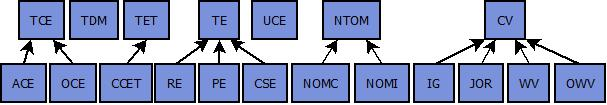
\includegraphics[width=3.1in]{images/MetricTaxonomy.jpg}
			%% Graphic for TeX using PGF
% Title: Z:\people\stephen\GlobalDocs\Projects\IPMAS\Architecture\Metric Taxonomy.dia
% Creator: Dia v0.97.2
% CreationDate: Thu Nov 01 16:39:04 2012
% For: stephen
% \usepackage{tikz}
% The following commands are not supported in PSTricks at present
% We define them conditionally, so when they are implemented,
% this pgf file will use them.
\ifx\du\undefined
  \newlength{\du}
\fi
\setlength{\du}{15\unitlength}
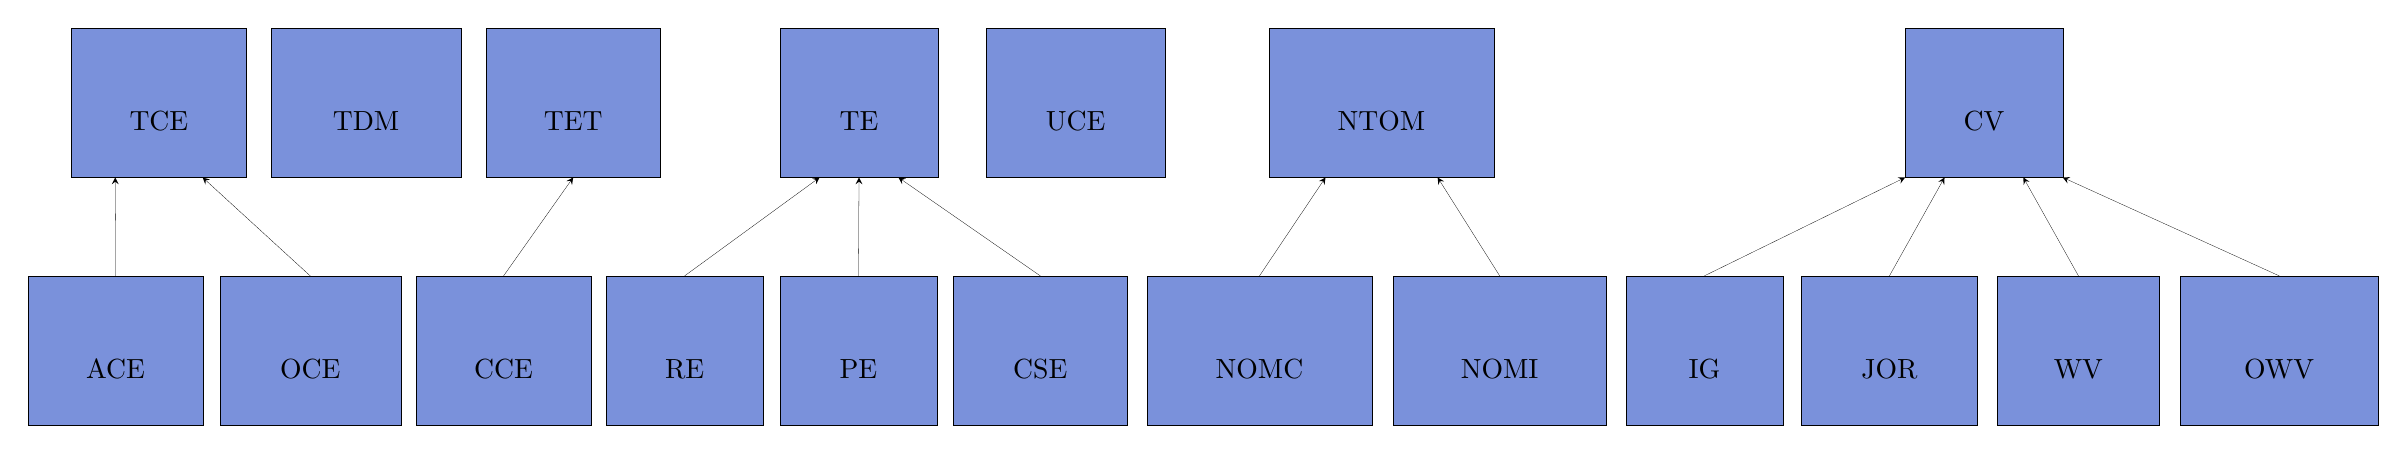
\begin{tikzpicture}
\pgftransformxscale{1.000000}
\pgftransformyscale{-1.000000}
\definecolor{dialinecolor}{rgb}{0.000000, 0.000000, 0.000000}
\pgfsetstrokecolor{dialinecolor}
\definecolor{dialinecolor}{rgb}{1.000000, 1.000000, 1.000000}
\pgfsetfillcolor{dialinecolor}
\definecolor{dialinecolor}{rgb}{0.478431, 0.568627, 0.858824}
\pgfsetfillcolor{dialinecolor}
\fill (1.257500\du,13.750000\du)--(1.257500\du,15.650000\du)--(3.487500\du,15.650000\du)--(3.487500\du,13.750000\du)--cycle;
\pgfsetlinewidth{0.100000\du}
\pgfsetdash{}{0pt}
\pgfsetdash{}{0pt}
\pgfsetmiterjoin
\definecolor{dialinecolor}{rgb}{0.000000, 0.000000, 0.000000}
\pgfsetstrokecolor{dialinecolor}
\draw (1.257500\du,13.750000\du)--(1.257500\du,15.650000\du)--(3.487500\du,15.650000\du)--(3.487500\du,13.750000\du)--cycle;
% setfont left to latex
\definecolor{dialinecolor}{rgb}{0.000000, 0.000000, 0.000000}
\pgfsetstrokecolor{dialinecolor}
\node at (2.372500\du,14.940000\du){ACE};
\definecolor{dialinecolor}{rgb}{0.478431, 0.568627, 0.858824}
\pgfsetfillcolor{dialinecolor}
\fill (3.694840\du,13.750000\du)--(3.694840\du,15.650000\du)--(5.992340\du,15.650000\du)--(5.992340\du,13.750000\du)--cycle;
\pgfsetlinewidth{0.100000\du}
\pgfsetdash{}{0pt}
\pgfsetdash{}{0pt}
\pgfsetmiterjoin
\definecolor{dialinecolor}{rgb}{0.000000, 0.000000, 0.000000}
\pgfsetstrokecolor{dialinecolor}
\draw (3.694840\du,13.750000\du)--(3.694840\du,15.650000\du)--(5.992340\du,15.650000\du)--(5.992340\du,13.750000\du)--cycle;
% setfont left to latex
\definecolor{dialinecolor}{rgb}{0.000000, 0.000000, 0.000000}
\pgfsetstrokecolor{dialinecolor}
\node at (4.843590\du,14.940000\du){OCE};
\definecolor{dialinecolor}{rgb}{0.478431, 0.568627, 0.858824}
\pgfsetfillcolor{dialinecolor}
\fill (1.812500\du,10.600000\du)--(1.812500\du,12.500000\du)--(4.032500\du,12.500000\du)--(4.032500\du,10.600000\du)--cycle;
\pgfsetlinewidth{0.100000\du}
\pgfsetdash{}{0pt}
\pgfsetdash{}{0pt}
\pgfsetmiterjoin
\definecolor{dialinecolor}{rgb}{0.000000, 0.000000, 0.000000}
\pgfsetstrokecolor{dialinecolor}
\draw (1.812500\du,10.600000\du)--(1.812500\du,12.500000\du)--(4.032500\du,12.500000\du)--(4.032500\du,10.600000\du)--cycle;
% setfont left to latex
\definecolor{dialinecolor}{rgb}{0.000000, 0.000000, 0.000000}
\pgfsetstrokecolor{dialinecolor}
\node at (2.922500\du,11.790000\du){TCE};
\definecolor{dialinecolor}{rgb}{0.478431, 0.568627, 0.858824}
\pgfsetfillcolor{dialinecolor}
\fill (4.352030\du,10.600000\du)--(4.352030\du,12.500000\du)--(6.754530\du,12.500000\du)--(6.754530\du,10.600000\du)--cycle;
\pgfsetlinewidth{0.100000\du}
\pgfsetdash{}{0pt}
\pgfsetdash{}{0pt}
\pgfsetmiterjoin
\definecolor{dialinecolor}{rgb}{0.000000, 0.000000, 0.000000}
\pgfsetstrokecolor{dialinecolor}
\draw (4.352030\du,10.600000\du)--(4.352030\du,12.500000\du)--(6.754530\du,12.500000\du)--(6.754530\du,10.600000\du)--cycle;
% setfont left to latex
\definecolor{dialinecolor}{rgb}{0.000000, 0.000000, 0.000000}
\pgfsetstrokecolor{dialinecolor}
\node at (5.553280\du,11.790000\du){TDM};
\definecolor{dialinecolor}{rgb}{0.478431, 0.568627, 0.858824}
\pgfsetfillcolor{dialinecolor}
\fill (7.074060\du,10.600000\du)--(7.074060\du,12.500000\du)--(9.294060\du,12.500000\du)--(9.294060\du,10.600000\du)--cycle;
\pgfsetlinewidth{0.100000\du}
\pgfsetdash{}{0pt}
\pgfsetdash{}{0pt}
\pgfsetmiterjoin
\definecolor{dialinecolor}{rgb}{0.000000, 0.000000, 0.000000}
\pgfsetstrokecolor{dialinecolor}
\draw (7.074060\du,10.600000\du)--(7.074060\du,12.500000\du)--(9.294060\du,12.500000\du)--(9.294060\du,10.600000\du)--cycle;
% setfont left to latex
\definecolor{dialinecolor}{rgb}{0.000000, 0.000000, 0.000000}
\pgfsetstrokecolor{dialinecolor}
\node at (8.184060\du,11.790000\du){TET};
\definecolor{dialinecolor}{rgb}{0.478431, 0.568627, 0.858824}
\pgfsetfillcolor{dialinecolor}
\fill (8.599690\du,13.750000\du)--(8.599690\du,15.650000\du)--(10.599690\du,15.650000\du)--(10.599690\du,13.750000\du)--cycle;
\pgfsetlinewidth{0.100000\du}
\pgfsetdash{}{0pt}
\pgfsetdash{}{0pt}
\pgfsetmiterjoin
\definecolor{dialinecolor}{rgb}{0.000000, 0.000000, 0.000000}
\pgfsetstrokecolor{dialinecolor}
\draw (8.599690\du,13.750000\du)--(8.599690\du,15.650000\du)--(10.599690\du,15.650000\du)--(10.599690\du,13.750000\du)--cycle;
% setfont left to latex
\definecolor{dialinecolor}{rgb}{0.000000, 0.000000, 0.000000}
\pgfsetstrokecolor{dialinecolor}
\node at (9.599690\du,14.940000\du){RE};
\definecolor{dialinecolor}{rgb}{0.478431, 0.568627, 0.858824}
\pgfsetfillcolor{dialinecolor}
\fill (10.807000\du,13.750000\du)--(10.807000\du,15.650000\du)--(12.807000\du,15.650000\du)--(12.807000\du,13.750000\du)--cycle;
\pgfsetlinewidth{0.100000\du}
\pgfsetdash{}{0pt}
\pgfsetdash{}{0pt}
\pgfsetmiterjoin
\definecolor{dialinecolor}{rgb}{0.000000, 0.000000, 0.000000}
\pgfsetstrokecolor{dialinecolor}
\draw (10.807000\du,13.750000\du)--(10.807000\du,15.650000\du)--(12.807000\du,15.650000\du)--(12.807000\du,13.750000\du)--cycle;
% setfont left to latex
\definecolor{dialinecolor}{rgb}{0.000000, 0.000000, 0.000000}
\pgfsetstrokecolor{dialinecolor}
\node at (11.807000\du,14.940000\du){PE};
\definecolor{dialinecolor}{rgb}{0.478431, 0.568627, 0.858824}
\pgfsetfillcolor{dialinecolor}
\fill (13.014400\du,13.750000\du)--(13.014400\du,15.650000\du)--(15.216900\du,15.650000\du)--(15.216900\du,13.750000\du)--cycle;
\pgfsetlinewidth{0.100000\du}
\pgfsetdash{}{0pt}
\pgfsetdash{}{0pt}
\pgfsetmiterjoin
\definecolor{dialinecolor}{rgb}{0.000000, 0.000000, 0.000000}
\pgfsetstrokecolor{dialinecolor}
\draw (13.014400\du,13.750000\du)--(13.014400\du,15.650000\du)--(15.216900\du,15.650000\du)--(15.216900\du,13.750000\du)--cycle;
% setfont left to latex
\definecolor{dialinecolor}{rgb}{0.000000, 0.000000, 0.000000}
\pgfsetstrokecolor{dialinecolor}
\node at (14.115650\du,14.940000\du){CSE};
\definecolor{dialinecolor}{rgb}{0.478431, 0.568627, 0.858824}
\pgfsetfillcolor{dialinecolor}
\fill (10.813600\du,10.600000\du)--(10.813600\du,12.500000\du)--(12.813600\du,12.500000\du)--(12.813600\du,10.600000\du)--cycle;
\pgfsetlinewidth{0.100000\du}
\pgfsetdash{}{0pt}
\pgfsetdash{}{0pt}
\pgfsetmiterjoin
\definecolor{dialinecolor}{rgb}{0.000000, 0.000000, 0.000000}
\pgfsetstrokecolor{dialinecolor}
\draw (10.813600\du,10.600000\du)--(10.813600\du,12.500000\du)--(12.813600\du,12.500000\du)--(12.813600\du,10.600000\du)--cycle;
% setfont left to latex
\definecolor{dialinecolor}{rgb}{0.000000, 0.000000, 0.000000}
\pgfsetstrokecolor{dialinecolor}
\node at (11.813600\du,11.790000\du){TE};
\definecolor{dialinecolor}{rgb}{0.478431, 0.568627, 0.858824}
\pgfsetfillcolor{dialinecolor}
\fill (13.433100\du,10.600000\du)--(13.433100\du,12.500000\du)--(15.698100\du,12.500000\du)--(15.698100\du,10.600000\du)--cycle;
\pgfsetlinewidth{0.100000\du}
\pgfsetdash{}{0pt}
\pgfsetdash{}{0pt}
\pgfsetmiterjoin
\definecolor{dialinecolor}{rgb}{0.000000, 0.000000, 0.000000}
\pgfsetstrokecolor{dialinecolor}
\draw (13.433100\du,10.600000\du)--(13.433100\du,12.500000\du)--(15.698100\du,12.500000\du)--(15.698100\du,10.600000\du)--cycle;
% setfont left to latex
\definecolor{dialinecolor}{rgb}{0.000000, 0.000000, 0.000000}
\pgfsetstrokecolor{dialinecolor}
\node at (14.565600\du,11.790000\du){UCE};
\pgfsetlinewidth{0.100000\du}
\pgfsetdash{}{0pt}
\pgfsetdash{}{0pt}
\pgfsetbuttcap
{
\definecolor{dialinecolor}{rgb}{0.000000, 0.000000, 0.000000}
\pgfsetfillcolor{dialinecolor}
% was here!!!
\pgfsetarrowsend{stealth}
\definecolor{dialinecolor}{rgb}{0.000000, 0.000000, 0.000000}
\pgfsetstrokecolor{dialinecolor}
\draw (2.372500\du,13.750000\du)--(2.367500\du,12.500000\du);
}
\pgfsetlinewidth{0.100000\du}
\pgfsetdash{}{0pt}
\pgfsetdash{}{0pt}
\pgfsetbuttcap
{
\definecolor{dialinecolor}{rgb}{0.000000, 0.000000, 0.000000}
\pgfsetfillcolor{dialinecolor}
% was here!!!
\pgfsetarrowsend{stealth}
\definecolor{dialinecolor}{rgb}{0.000000, 0.000000, 0.000000}
\pgfsetstrokecolor{dialinecolor}
\draw (4.843590\du,13.750000\du)--(3.477500\du,12.500000\du);
}
\pgfsetlinewidth{0.100000\du}
\pgfsetdash{}{0pt}
\pgfsetdash{}{0pt}
\pgfsetbuttcap
{
\definecolor{dialinecolor}{rgb}{0.000000, 0.000000, 0.000000}
\pgfsetfillcolor{dialinecolor}
% was here!!!
\pgfsetarrowsend{stealth}
\definecolor{dialinecolor}{rgb}{0.000000, 0.000000, 0.000000}
\pgfsetstrokecolor{dialinecolor}
\draw (9.599690\du,13.750000\du)--(11.313600\du,12.500000\du);
}
\pgfsetlinewidth{0.100000\du}
\pgfsetdash{}{0pt}
\pgfsetdash{}{0pt}
\pgfsetbuttcap
{
\definecolor{dialinecolor}{rgb}{0.000000, 0.000000, 0.000000}
\pgfsetfillcolor{dialinecolor}
% was here!!!
\pgfsetarrowsend{stealth}
\definecolor{dialinecolor}{rgb}{0.000000, 0.000000, 0.000000}
\pgfsetstrokecolor{dialinecolor}
\draw (11.807000\du,13.750000\du)--(11.813600\du,12.500000\du);
}
\pgfsetlinewidth{0.100000\du}
\pgfsetdash{}{0pt}
\pgfsetdash{}{0pt}
\pgfsetbuttcap
{
\definecolor{dialinecolor}{rgb}{0.000000, 0.000000, 0.000000}
\pgfsetfillcolor{dialinecolor}
% was here!!!
\pgfsetarrowsend{stealth}
\definecolor{dialinecolor}{rgb}{0.000000, 0.000000, 0.000000}
\pgfsetstrokecolor{dialinecolor}
\draw (14.115650\du,13.750000\du)--(12.313600\du,12.500000\du);
}
\definecolor{dialinecolor}{rgb}{0.478431, 0.568627, 0.858824}
\pgfsetfillcolor{dialinecolor}
\fill (6.185000\du,13.750000\du)--(6.185000\du,15.650000\du)--(8.415000\du,15.650000\du)--(8.415000\du,13.750000\du)--cycle;
\pgfsetlinewidth{0.100000\du}
\pgfsetdash{}{0pt}
\pgfsetdash{}{0pt}
\pgfsetmiterjoin
\definecolor{dialinecolor}{rgb}{0.000000, 0.000000, 0.000000}
\pgfsetstrokecolor{dialinecolor}
\draw (6.185000\du,13.750000\du)--(6.185000\du,15.650000\du)--(8.415000\du,15.650000\du)--(8.415000\du,13.750000\du)--cycle;
% setfont left to latex
\definecolor{dialinecolor}{rgb}{0.000000, 0.000000, 0.000000}
\pgfsetstrokecolor{dialinecolor}
\node at (7.300000\du,14.940000\du){CCE};
\pgfsetlinewidth{0.100000\du}
\pgfsetdash{}{0pt}
\pgfsetdash{}{0pt}
\pgfsetbuttcap
{
\definecolor{dialinecolor}{rgb}{0.000000, 0.000000, 0.000000}
\pgfsetfillcolor{dialinecolor}
% was here!!!
\pgfsetarrowsend{stealth}
\definecolor{dialinecolor}{rgb}{0.000000, 0.000000, 0.000000}
\pgfsetstrokecolor{dialinecolor}
\draw (7.300000\du,13.750000\du)--(8.184060\du,12.500000\du);
}
\definecolor{dialinecolor}{rgb}{0.478431, 0.568627, 0.858824}
\pgfsetfillcolor{dialinecolor}
\fill (15.471250\du,13.750000\du)--(15.471250\du,15.650000\du)--(18.328750\du,15.650000\du)--(18.328750\du,13.750000\du)--cycle;
\pgfsetlinewidth{0.100000\du}
\pgfsetdash{}{0pt}
\pgfsetdash{}{0pt}
\pgfsetmiterjoin
\definecolor{dialinecolor}{rgb}{0.000000, 0.000000, 0.000000}
\pgfsetstrokecolor{dialinecolor}
\draw (15.471250\du,13.750000\du)--(15.471250\du,15.650000\du)--(18.328750\du,15.650000\du)--(18.328750\du,13.750000\du)--cycle;
% setfont left to latex
\definecolor{dialinecolor}{rgb}{0.000000, 0.000000, 0.000000}
\pgfsetstrokecolor{dialinecolor}
\node at (16.900000\du,14.940000\du){NOMC};
\definecolor{dialinecolor}{rgb}{0.478431, 0.568627, 0.858824}
\pgfsetfillcolor{dialinecolor}
\fill (18.593750\du,13.750000\du)--(18.593750\du,15.650000\du)--(21.306250\du,15.650000\du)--(21.306250\du,13.750000\du)--cycle;
\pgfsetlinewidth{0.100000\du}
\pgfsetdash{}{0pt}
\pgfsetdash{}{0pt}
\pgfsetmiterjoin
\definecolor{dialinecolor}{rgb}{0.000000, 0.000000, 0.000000}
\pgfsetstrokecolor{dialinecolor}
\draw (18.593750\du,13.750000\du)--(18.593750\du,15.650000\du)--(21.306250\du,15.650000\du)--(21.306250\du,13.750000\du)--cycle;
% setfont left to latex
\definecolor{dialinecolor}{rgb}{0.000000, 0.000000, 0.000000}
\pgfsetstrokecolor{dialinecolor}
\node at (19.950000\du,14.940000\du){NOMI};
\definecolor{dialinecolor}{rgb}{0.478431, 0.568627, 0.858824}
\pgfsetfillcolor{dialinecolor}
\fill (17.026250\du,10.600000\du)--(17.026250\du,12.500000\du)--(19.873750\du,12.500000\du)--(19.873750\du,10.600000\du)--cycle;
\pgfsetlinewidth{0.100000\du}
\pgfsetdash{}{0pt}
\pgfsetdash{}{0pt}
\pgfsetmiterjoin
\definecolor{dialinecolor}{rgb}{0.000000, 0.000000, 0.000000}
\pgfsetstrokecolor{dialinecolor}
\draw (17.026250\du,10.600000\du)--(17.026250\du,12.500000\du)--(19.873750\du,12.500000\du)--(19.873750\du,10.600000\du)--cycle;
% setfont left to latex
\definecolor{dialinecolor}{rgb}{0.000000, 0.000000, 0.000000}
\pgfsetstrokecolor{dialinecolor}
\node at (18.450000\du,11.790000\du){NTOM};
\definecolor{dialinecolor}{rgb}{0.478431, 0.568627, 0.858824}
\pgfsetfillcolor{dialinecolor}
\fill (21.550000\du,13.750000\du)--(21.550000\du,15.650000\du)--(23.550000\du,15.650000\du)--(23.550000\du,13.750000\du)--cycle;
\pgfsetlinewidth{0.100000\du}
\pgfsetdash{}{0pt}
\pgfsetdash{}{0pt}
\pgfsetmiterjoin
\definecolor{dialinecolor}{rgb}{0.000000, 0.000000, 0.000000}
\pgfsetstrokecolor{dialinecolor}
\draw (21.550000\du,13.750000\du)--(21.550000\du,15.650000\du)--(23.550000\du,15.650000\du)--(23.550000\du,13.750000\du)--cycle;
% setfont left to latex
\definecolor{dialinecolor}{rgb}{0.000000, 0.000000, 0.000000}
\pgfsetstrokecolor{dialinecolor}
\node at (22.550000\du,14.940000\du){IG};
\definecolor{dialinecolor}{rgb}{0.478431, 0.568627, 0.858824}
\pgfsetfillcolor{dialinecolor}
\fill (23.783750\du,13.750000\du)--(23.783750\du,15.650000\du)--(26.016250\du,15.650000\du)--(26.016250\du,13.750000\du)--cycle;
\pgfsetlinewidth{0.100000\du}
\pgfsetdash{}{0pt}
\pgfsetdash{}{0pt}
\pgfsetmiterjoin
\definecolor{dialinecolor}{rgb}{0.000000, 0.000000, 0.000000}
\pgfsetstrokecolor{dialinecolor}
\draw (23.783750\du,13.750000\du)--(23.783750\du,15.650000\du)--(26.016250\du,15.650000\du)--(26.016250\du,13.750000\du)--cycle;
% setfont left to latex
\definecolor{dialinecolor}{rgb}{0.000000, 0.000000, 0.000000}
\pgfsetstrokecolor{dialinecolor}
\node at (24.900000\du,14.940000\du){JOR};
\definecolor{dialinecolor}{rgb}{0.478431, 0.568627, 0.858824}
\pgfsetfillcolor{dialinecolor}
\fill (26.268750\du,13.750000\du)--(26.268750\du,15.650000\du)--(28.331250\du,15.650000\du)--(28.331250\du,13.750000\du)--cycle;
\pgfsetlinewidth{0.100000\du}
\pgfsetdash{}{0pt}
\pgfsetdash{}{0pt}
\pgfsetmiterjoin
\definecolor{dialinecolor}{rgb}{0.000000, 0.000000, 0.000000}
\pgfsetstrokecolor{dialinecolor}
\draw (26.268750\du,13.750000\du)--(26.268750\du,15.650000\du)--(28.331250\du,15.650000\du)--(28.331250\du,13.750000\du)--cycle;
% setfont left to latex
\definecolor{dialinecolor}{rgb}{0.000000, 0.000000, 0.000000}
\pgfsetstrokecolor{dialinecolor}
\node at (27.300000\du,14.940000\du){WV};
\definecolor{dialinecolor}{rgb}{0.478431, 0.568627, 0.858824}
\pgfsetfillcolor{dialinecolor}
\fill (28.593750\du,13.750000\du)--(28.593750\du,15.650000\du)--(31.106250\du,15.650000\du)--(31.106250\du,13.750000\du)--cycle;
\pgfsetlinewidth{0.100000\du}
\pgfsetdash{}{0pt}
\pgfsetdash{}{0pt}
\pgfsetmiterjoin
\definecolor{dialinecolor}{rgb}{0.000000, 0.000000, 0.000000}
\pgfsetstrokecolor{dialinecolor}
\draw (28.593750\du,13.750000\du)--(28.593750\du,15.650000\du)--(31.106250\du,15.650000\du)--(31.106250\du,13.750000\du)--cycle;
% setfont left to latex
\definecolor{dialinecolor}{rgb}{0.000000, 0.000000, 0.000000}
\pgfsetstrokecolor{dialinecolor}
\node at (29.850000\du,14.940000\du){OWV};
\definecolor{dialinecolor}{rgb}{0.478431, 0.568627, 0.858824}
\pgfsetfillcolor{dialinecolor}
\fill (25.100000\du,10.600000\du)--(25.100000\du,12.500000\du)--(27.100000\du,12.500000\du)--(27.100000\du,10.600000\du)--cycle;
\pgfsetlinewidth{0.100000\du}
\pgfsetdash{}{0pt}
\pgfsetdash{}{0pt}
\pgfsetmiterjoin
\definecolor{dialinecolor}{rgb}{0.000000, 0.000000, 0.000000}
\pgfsetstrokecolor{dialinecolor}
\draw (25.100000\du,10.600000\du)--(25.100000\du,12.500000\du)--(27.100000\du,12.500000\du)--(27.100000\du,10.600000\du)--cycle;
% setfont left to latex
\definecolor{dialinecolor}{rgb}{0.000000, 0.000000, 0.000000}
\pgfsetstrokecolor{dialinecolor}
\node at (26.100000\du,11.790000\du){CV};
\pgfsetlinewidth{0.100000\du}
\pgfsetdash{}{0pt}
\pgfsetdash{}{0pt}
\pgfsetbuttcap
{
\definecolor{dialinecolor}{rgb}{0.000000, 0.000000, 0.000000}
\pgfsetfillcolor{dialinecolor}
% was here!!!
\pgfsetarrowsend{stealth}
\definecolor{dialinecolor}{rgb}{0.000000, 0.000000, 0.000000}
\pgfsetstrokecolor{dialinecolor}
\draw (16.900000\du,13.750000\du)--(17.738125\du,12.500000\du);
}
\pgfsetlinewidth{0.100000\du}
\pgfsetdash{}{0pt}
\pgfsetdash{}{0pt}
\pgfsetbuttcap
{
\definecolor{dialinecolor}{rgb}{0.000000, 0.000000, 0.000000}
\pgfsetfillcolor{dialinecolor}
% was here!!!
\pgfsetarrowsend{stealth}
\definecolor{dialinecolor}{rgb}{0.000000, 0.000000, 0.000000}
\pgfsetstrokecolor{dialinecolor}
\draw (19.950000\du,13.750000\du)--(19.161875\du,12.500000\du);
}
\pgfsetlinewidth{0.100000\du}
\pgfsetdash{}{0pt}
\pgfsetdash{}{0pt}
\pgfsetbuttcap
{
\definecolor{dialinecolor}{rgb}{0.000000, 0.000000, 0.000000}
\pgfsetfillcolor{dialinecolor}
% was here!!!
\pgfsetarrowsend{stealth}
\definecolor{dialinecolor}{rgb}{0.000000, 0.000000, 0.000000}
\pgfsetstrokecolor{dialinecolor}
\draw (22.550000\du,13.750000\du)--(25.100000\du,12.500000\du);
}
\pgfsetlinewidth{0.100000\du}
\pgfsetdash{}{0pt}
\pgfsetdash{}{0pt}
\pgfsetbuttcap
{
\definecolor{dialinecolor}{rgb}{0.000000, 0.000000, 0.000000}
\pgfsetfillcolor{dialinecolor}
% was here!!!
\pgfsetarrowsend{stealth}
\definecolor{dialinecolor}{rgb}{0.000000, 0.000000, 0.000000}
\pgfsetstrokecolor{dialinecolor}
\draw (24.900000\du,13.750000\du)--(25.600000\du,12.500000\du);
}
\pgfsetlinewidth{0.100000\du}
\pgfsetdash{}{0pt}
\pgfsetdash{}{0pt}
\pgfsetbuttcap
{
\definecolor{dialinecolor}{rgb}{0.000000, 0.000000, 0.000000}
\pgfsetfillcolor{dialinecolor}
% was here!!!
\pgfsetarrowsend{stealth}
\definecolor{dialinecolor}{rgb}{0.000000, 0.000000, 0.000000}
\pgfsetstrokecolor{dialinecolor}
\draw (27.300000\du,13.750000\du)--(26.600000\du,12.500000\du);
}
\pgfsetlinewidth{0.100000\du}
\pgfsetdash{}{0pt}
\pgfsetdash{}{0pt}
\pgfsetbuttcap
{
\definecolor{dialinecolor}{rgb}{0.000000, 0.000000, 0.000000}
\pgfsetfillcolor{dialinecolor}
% was here!!!
\pgfsetarrowsend{stealth}
\definecolor{dialinecolor}{rgb}{0.000000, 0.000000, 0.000000}
\pgfsetstrokecolor{dialinecolor}
\draw (29.850000\du,13.750000\du)--(27.100000\du,12.500000\du);
}
\end{tikzpicture}
}
		\end{center}

	\caption{Kitting static metric taxonomy with abbreviations defined below}
	\label{fig:StaticMetricTax}
\end{figure}

The current metric taxonomy is shown in Figure~\ref{fig:StaticMetricTax} and is
described below. The metrics are designed to be evaluated at the end of each
CRCL command with cumulative values.

\begin{itemize}

\item \sf Action Commands Executed (ACE) \rm -- the number of action commands that
  have been executed so far. An action command is any command that takes
  time to execute.\\

\item \sf Command Sequence Errors (CSE) \rm -- the number of commands that are
  out of sequence. An InitCanon command is out of sequence if it is not the
  first command in the file. An EndCanon command is out of sequence if it
  is not the last command in the file. Other commands are out of sequence
  if they occur before InitCanon or after EndCanon.\\

\item \sf Constraint Violations (CV) \rm -- the total of IG, JOR, WV and OWV.\\

\item \sf Current Command Execution Time (CCET) \rm -- the time that the current
   command took to execute.\\

\item \sf Incorrect Gripper (IG) \rm -- the wrong gripper was used to pick up an object.\\

\item \sf Joint Out of Range (JOR) \rm -- a joint of the robot was commanded to
  move to an out-of-limit position.\\

\item \sf Number of Objects Moved Correctly (NOMC) \rm -- the number of objects
  that were moved correctly from the parts supply to the kit.\\

\item \sf Number of Objects Moved Incorrectly (NOMI) \rm -- the number of objects
  that were moved to an incorrect position in the kit.\\

\item \sf Number of Total Objects Moved (NTOM) \rm -- the sum of NOMC and NOMI.\\

\item \sf Other Commands Executed (OCE) \rm -- the number of commands that are
  not action commands that have been executed so far -- mostly setting
  commands. Executing these commands is assumed to take a negligible amount
  of time.\\

\item \sf Outside Work Volume (OWV) \rm -- the robot was asked to move outside its
  work volume.\\

\item \sf Parse Errors  (PE) \rm -- the number of lines in the CRCL command file
  that cause an error in the command file parser. \\

\item \sf Range Errors (RE) \rm -- the number of times a command tries to set a
  a parameter to a value that is out of the allowed range of the parameter.\\

 \item \sf Total Commands Executed (TCE) \rm -- the sum of ACE and OCE.\\

\item \sf Total Distance Moved (TDM) \rm -- the total distance that the
  tool tip has moved.  This is calculated as the total of the distances between
  points in
  the move commands, taken in order (and starting at the place where the
  controlled point is located initially). The value is updated as each point
  is reached, not continuously.\\

\item \sf Total Execution Time (TET) \rm -- the total time taken so far by
  executing action commands. This does not include any time that may elapse
  between when one command finishes execution and when the user tells the
  system to execute another command. The total execution time is
  meant to be very close to the actual amount of time that would be taken
  by the system without user intervention.\\

\item \sf Total Errors (TE) \rm -- the sum of the range errors, parse errors,
  and command sequence errors.\\

\item \sf Useless Command Executed (UCE) \rm -- the number of commands that do
  not change the state of the workstation. Such commands have no effect, so
  they are useless. The \sf CloseGripper() \rm and \sf CloseToolChanger()
  \rm commands in Figure~\ref{fig:KittingPlan} are useless because the
  gripper and tool changer are closed in the initial conditions.\\

\item \sf Weight Violation (WV) \rm -- the robot was asked to move some object that
  violates its load capacity.

\end{itemize}

\subsection{Execution Metrics for Kit Building}
During execution, automated kitting fails to reach its full potential when the supply chain fails and parts and components are not available for kit construction, or when a kit is not properly filled. Part availability failures can be triggered by inaccurate information about the location of the part or part shortage due to delays in internal logistics. Kit construction errors may be due to problems such as improper equipment setup, improper equipment maintenance, part damage, wrong type of part, or part dropped by the robot.


Models for detecting and recovering from plan execution failures mostly deal with \textit{precondition failures}, \textit{action failures}, and \textit{unattributable failures}~\cite{Myers1998}. Precondition failures appear when all the preconditions for an action are not met during the execution of the action. Action failures are encountered when the execution of an action does not attain its intended effects. Unattributable failures occur when unexpected events caused by external agents change the environment, thus causing the current plan to become obsolete. NIST\rq{}s Knowledge Driven Planning and Modeling project has not yet addressed the creation of a taxonomy of  execution errors. However, some preliminary metrics have been developed and are described
below.

\begin{itemize}
\item \sf Manipulation robustness \rm -- quantitative and qualitative functionality metrics that describe how well a robot can handle complex objects in complex environments without failing or requiring additional operator interventions. Failures can occur during object detection (lightning variation, shadows), object approach (partially buried), and object manipulation (fragile) operations.
It is envisioned that a taxonomy of robustness will be developed that decomposes robustness into areas such as situational awareness, robot accuracy, and grasping dexterity.\\

\item \sf Transporting components \rm -- qualitative metrics that describe how well a robotic arm can grasp objects and move these objects from an initial position to a goal position without dropping them.\\

\item \sf Plan generation \rm -- as mentioned previously, failures are possible in kitting during the execution of CRCL commands, causing the current plan to become obsolete. In some cases, the current state of the environment is brought back to the state prior to the failure and the robot starts from a ``stable" state. In other cases, a completely new plan must be generated by the planning system where the robot starts all over. This metric will measure the planning system\rq{}s ability to adapt to failures.\\

\item \sf Contact errors \rm -- quantitative metrics that keep track of the number of collisions between the robotic arm and objects in the environment. The performance of the robotic arm during kit building is affected by the positions of joints and the end-effector in the environment. The position of the end-effector can reduce the time to complete tasks but can also increase the number of collisions due to joint contact with other objects in a confined space.\\

\item \sf Failures during kit building\rm -- quantitative metrics that report the total number of failures encountered during kit building. When a failure occurs during the
building of a kit, the number of failures is increased by one. The system may generate a new plan to recover from the failure. If a failure occurs during the execution of the new
plan, the number of failures in increased by one again.\\

\item \sf Failure modes recovery \rm -- quantitative metrics that represent the number of failure modes the system recovers from through the use of contingency plans. When a failure is detected in the execution process, failure monitors encode appropriate responses (contingency plans) to failure modes for this particular failure.\\

\end{itemize}


%%%%%%%%%%%%%%%%%%%%%%%%%%%%%%%%%%%%%%%%%%%%%%%%%%%%%%%%%%%%
\section{Kitting Viewer}
\label{sect:KittingViewer}
A software tool named the ``Kitting Viewer'' has been developed that
simulates the execution of a plan (CRCL command file) for changing a
kitting workstation from an initial state to a goal state. Usually, that is
a plan for making one or more kits. The Kitting Viewer evaluates the plan
as it runs. The Kitting Viewer source code is in C++ with OpenGL\footnote{Certain commercial/open source software and tools are identified in this paper in order to explain our research. Such identification does not imply
recommendation or endorsement by the authors or NIST, nor does it imply that the software tools identified are necessarily the best available for the purpose.} graphics.

\begin{figure}[ht!]
\centering
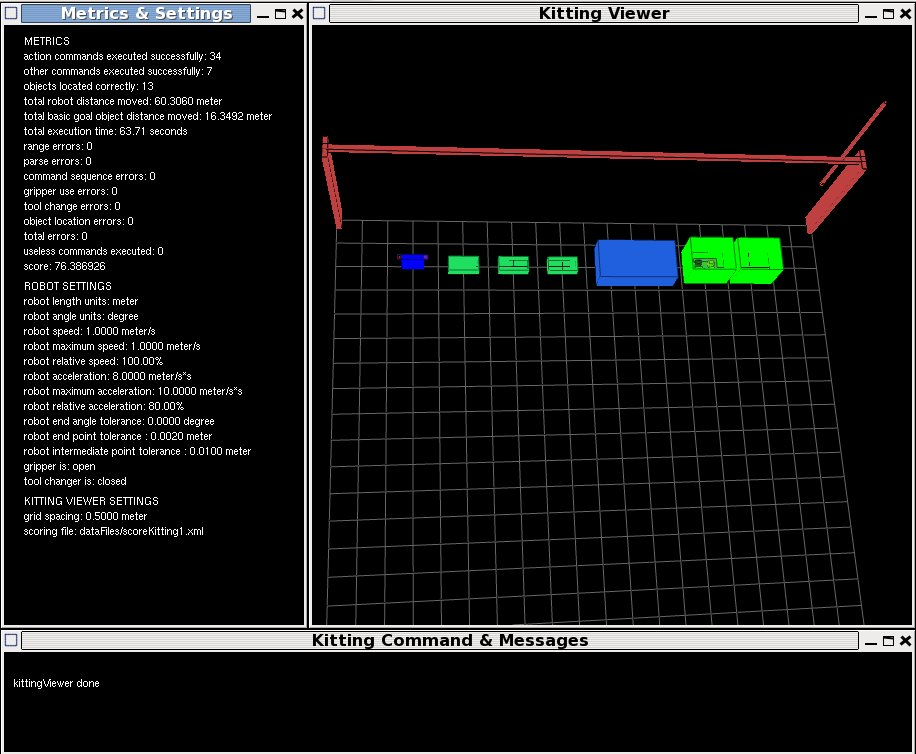
\includegraphics[width=8.5cm]{images/kittingViewer2013Feb23.jpg}
\caption{Kitting Viewer Display}
\label{fig:KittingViewer}
\end{figure}

\subsection{Overview}

The Kitting Viewer reads files describing the initial state, the goal
state, and the plan for getting from the initial state to the goal state.
Optionally, it also reads a scoring file. If no scoring file is specified
by the user, a hard-coded default scoring file structure is used. The
Kitting Viewer simulates execution of the plan, displays a view of the plan
being executed, and produces and displays metrics about the plan. All of
the metrics are numbers. All but one of the metrics are objective and
require no human judgement. These metrics are presented in Section
\ref{sect:Metrics}. The final metric is a subjective combination of the
other metrics in which the other metrics are weighted and combined as
specified by the scoring file. The scoring file may be edited as desired by
the user. Scoring details are given in Section \ref{sect:Scoring}.

Controlling the Kitting Viewer is accomplished by using the mouse and single
keys on the keyboard. When the Kitting Viewer starts up, a set of one-line
instructions is printed in the terminal window from which the
Kitting Viewer was started.

The Kitting Viewer runs in two phases. In the first phase, each time the
user gives a signal (presses the \tt g \rm key) the next command from the
command file is executed. The Kitting Viewer may decide that a command
cannot be executed, but if it decides a command can be executed, it assumes
the command is executed properly. In the second phase, which starts after
all commands have been executed, each time the user gives a signal the
position of the next movable object in the goal file is checked.

Figure~\ref{fig:KittingViewer} shows the Kitting Viewer windows as they
look after a test run has been completed. The display uses three windows,
labeled Metrics \& Settings, Kitting Viewer, and Kitting Command \&
Messages. The windows may be moved and re-sized independently, like other
windows in a typical windowing system. At any time, the user may save a
combined image of all three windows in a file in portable pixmap (.ppm)
format, a common graphics format that many graphics utilities can handle.

In Figure~\ref{fig:KittingViewer}, the large blue object is a work table.
The small blue object is the end effector changing station. The three empty
small green boxes are parts trays that formerly held parts. The large green
box on the left is a container for completed kits; it contains one kit. The
large empty green box on the right formerly held an empty kit tray.

The Kitting Viewer window shows a 3D animated color view of the kitting
workstation. The floor of the workstation is covered with a grid. The robot
in the workstation is represented by a gantry robot spanning the entire
width of the workstation. The gantry robot moves when any CRCL motion
command is executed. The speed at which the picture of the robot is
animated matches the actual commanded speed of the robot. Objects in the
workstation move if the robot moves them. The view in the window may be
translated, rotated, or zoomed at any time.

In the first phase of running the Kitting Viewer, the Kitting Command \&
Messages window shows the currently executing command or the most recently
executed command, if no command is currently executing. In the second
phase, the window shows messages describing success or failure in locating
goal objects.

The Metrics \& Settings window shows 12 (first phase) or 15 (second phase)
metrics at the top. Below that it shows 13 robot settings and two
Kitting Viewer settings. All but two of the robot settings correspond to
items that may be set using CRCL commands. The extra two are the
robot\rq{}s maximum speed and maximum acceleration, which may not be
reset. As commands are executed, metrics and settings are updated in the
window.

\subsection{Errors}
In order to fully evaluate a plan file, usually, if a plan error is
detected, an error is recorded, but the Kitting Viewer continues to operate.
A few errors are fatal.
  
When the command parser encounters a line that it cannot parse, it adds
an \sf UnreadableMsg \rm to the list of commands it has parsed. The \sf
UnreadableMsg \rm includes the text of the line on which the parse error
occurred. When the \sf UnreadableMsg \rm is executed, the value of parse
errors is increased by one and the \sf UnreadableMsg \rm is displayed in
the Kitting Command \& Messages window so the user can see the line that
caused the problem.

\subsection{Modeling}
The project in which the Kitting Viewer was developed has modeled the state
of a kitting workstation in both OWL and XML schema language. The XML model
is kitting.xsd. An automatic code generator named the GenXMiller written by
the authors at NIST is being used in the project. The GenXMiller will read
an XML schema and produce C++ classes and a parser for XML data files
corresponding to the XML schema. The GenXMiller was used to produce the C++
class model of a kitting workstation and the state file parser used in the
Kitting Viewer. The initial and goal state files used by the Kitting Viewer
are XML data files corresponding to the kitting.xsd XML schema.

The Kitting Viewer does a great deal of modeling while it runs. When the
initial state file is read, a model of the initial state is built and saved
as the current state of the workstation. A model of the goal state is also
built and saved. As the Kitting Viewer runs and CRCL commands are executed,
the Kitting Viewer determines the effect of executing each command on the
current state and updates it. The second phase of Kitting Viewer operation
compares the evolved current state with the goal state.

The logic of state changes is complex in some cases. The most interesting
cases involve what to do when executing CloseGripper and OpenGripper
commands. Details for CloseGripper are given below. 

A key issue is that composite objects may go out of existence or come into
existence while kits are being built. A kitting workstation builds kits.
The kits do not exist in the initial state but they do exist in the goal
state, so it is necessary to make them start to exist at some point in the
process. The initial state includes parts trays with parts. When all the
parts are removed from a parts tray with parts, it goes out of existence.
Of course the parts tray remains, but it is no longer a component of a
parts tray with parts. In the Kitting Viewer, a kit comes into existence
when the first part is placed in a kit tray, and a parts tray with parts
goes out of existence when the last part is removed from it.

For CloseGripper, if all of the following hold:
\newcounter{ifcount}
\begin{list}{\arabic{ifcount}.}%
{\usecounter{ifcount}}

\item  The robot is holding an end effector.

\item  The end effector is a single cup vacuum gripper (that's the only
   kind of gripper the Kitting Viewer knows how to use).

\item Either:\\
3a. There is a parts tray or kit tray with a topless boxy shape
    such that the gripper cup is within 0.1 mm of the bottom of the
    tray and is within 1 mm of the XY location of the origin of the tray. OR\\
3b. There is a part with a boxy shape with top such that the gripper cup
    is within 0.1 mm of the top of the part and is within 1 mm of the XY
    location of the middle of the top of the part.

\item The gripper is able to pick up that type of part or tray.

\item The Z axis of the gripper is 0,0,-1 and the Z axis of the object is
    0,0,1.

\item The gripper is open (implying the gripper is not holding anything).

\end{list}

Then the gripper will attach to an object. Call it B.

\begin{itemize}

\item If 3b above occurred, then B is a part

\item If 3a above occurred with a parts tray in a parts tray with parts,
   then B is the parts tray with parts.

\item If 3a above occurred with a parts tray not in a parts tray with parts,
   then B is the parts tray.

\item If 3a above occurred with a kit tray in a kit, then B is the kit.

\item If 3a above occurred with a kit tray not in a kit, then B is the kit tray.

\end{itemize}

When the gripper attaches to an object, the primary state changes (i.e.
changes in states present in kitting.xsd) are that the gripper is closed,
and the pose of the object is changed so that the object is located
relative to the gripper. In addition, as described above, if the object is
the last part in a parts tray with parts, the parts tray with parts will go
out of existence. The Kitting Viewer has several other state variables for
positions to make its work more efficient, and these are also updated.



%%%%%%%%%%%%%%%%%%%%%%%%%%%%%%%%%%%%%%%%%%%%%%%%%%%%%%%%%%%%

\addtolength{\textheight}{-4cm}
                                  % This command serves to balance the column lengths
                                  % on the last page of dthe document manually. It shortens
                                  % the textheight of the last page by a suitable amount.
                                  % This command does not take effect until the next page
                                  % so it should come on the page before the last. Make
                                  % sure that you do not shorten the textheight too much.

%%%%%%%%%%%%%%%%%%%%%%%%%%%%%%%%%%%%%%%%%%%%%%%%%%%%%%%%%%%%%%%%%%%%%%%%%%%%%%%%

%%%%%%%%%%%%%%%%%%%%%%%%%%%%%%%%%%%%%%%%%%%%%%%%%%%%%%%%%%%%
\section{CONCLUSIONS AND FUTURE WORK}
\label{sect:Conclusions}
The IPMAS project is scheduled to continue for an additional two years. During this time,
we hope to improve on all aspects of the knowledge representation and standardization
effort. These improvements include increased outreach to industry, improvement on
test methods and metrics, and improvements on our ontology and knowledge
representation that will be fed to the IEEE working group.

\subsection{Kitting Viewer Development Plans}

As mentioned earlier, the kittingViewer is far from complete. It is
planned to add the following capabilities.

\begin{itemize}

\item Add drawing the kitting workstation in its current state. The initial
  state of the workstation is already available in data as soon as the XML
  data file that describes it is read in.

\item Add updating the positions of objects as the robot executes commands.
  It will be necessary to compare the position of the robot with the
  positions of objects when OpenGripper and CloseGripper commands are
  executed in order to determine if the robot is grasping them.

\item Add metrics related to the positions of objects. This might include
  (1) the number of objects that should have been moved, (2) the number of
  objects that were moved, (3) the number of objects that were moved to the
  correct place, (4) the number of objects that were moved to the wrong
  place.

\item Add metrics related to constraint violations. This might include (1)
  the number of instances of picking up an object that weighs more than the
  robot's load capacity, (2) the number of instances of the robot moving
  outside of its work volume, (3) the number of instances of using a
  gripper to move an object when the gripper is not qualified to move the
  object. It will also be necessary to decide what the simulation should do
  in these cases and implement that.

\item Add a total score metric, and implement finding the total score using
  a configuration file in which the user assigns weights to the other
  metrics.
\end{itemize} 

\subsection{Ontology Development Plans}
We have created a knowledge driven system that is capable of building
kits in a flexible and agile manor assuming perfect actions. For this system
to be practical, this restriction must be removed. 
To enable this, our current work on the development of a taxonomy of
predicates for the situational awareness necessary for kit building will
be continued and expanded. The system will also be augmented to
allow for the checking of necessary preconditions before actions are
executed, and the verification of results after an action has occurred.

To date, we have developed a knowledge representation that supports
kitting operations. In cooperation with the IEEE Working Group, this
representation will be expanded to support general assembly operations.
In addition, we will work with the IEEE Working Group, academia, and 
industry to standardize the knowledge representations, test methods,
and metrics.


\bibliographystyle{asmems4}
\bibliography{kitting}
\end{document}
